\documentclass[letterpaper,12pt,leqno]{article}
\usepackage{paper}
\usepackage{authblk}
\bibliographystyle{apalike}
\usepackage{math}
\hypersetup{
  colorlinks=true,
  linkcolor=blue,
  filecolor=magenta,
  urlcolor=blue,
  citecolor=blue
}
\graphicspath{{DATI/}}
\title{The spatial diffusion of the British Industrial Revolution: Evidence from patent geography}
\author[1]{Nicol\`o Badino}
\affil[1]{Department of Economics, University of Genova}
\date{\today}
\setcounter{Maxaffil}{0}
\renewcommand\Affilfont{\itshape\small}
\begin{document}
\maketitle
\begin{abstract}
  This study traces the spatial diffusion of formalized inventive activity across Europe using newly available patent data from the PatentCity database, treating the geography of patents as a proxy for the spread of industrialization. We introduce a spatiotemporal extension of kernel density estimation (KDE) to construct diffusion waves of patenting intensity that proxy the timing and location of industrial take-off at the regional level. Combined with a gravity model of knowledge spillovers and a Cox proportional hazards model, our analysis yields three main findings. First, the industrialization of continental Europe followed a wave-like diffusion process with a strong spatial component: proximity to the British epicenter, measured through historical transport networks, was the dominant predictor of both innovation intensity and timing. Second, structural estimation reveals that knowledge spillovers operated with diminishing returns to accumulated knowledge and were primarily a ``push'' phenomenon driven by source-region population, while receiving-region size played no amplifying role.
\end{abstract}

%\noindent\textbf{JEL Classification:} N13, O33, R12, F63

%\noindent\textbf{Keywords:} Industrial Revolution, Technology Diffusion, Spatial Economics, Patents, Knowledge Spillovers

\section{Introduction}

The causes and consequences of the British Industrial Revolution have been studied in depth, but the spatial dynamics of its diffusion across continental Europe have received comparatively less attention. This study investigates the geographical spread of formalized inventive activity, as captured by patent filings, from Great Britain to continental Europe during the 19th century, interpreting patent geography as a proxy for the broader process of industrialization.
The Industrial Revolution coincides with the period in which European patent systems became more observable and systematically documentable; patents are therefore a particularly useful source for spatiotemporal analysis of innovation, even though patent statutes existed earlier (e.g., the Venetian Statute of 1474 or the English Statute of Monopolies of 1624).
We focus primarily on the European case, positing that the diffusion of registered inventive knowledge followed a spatial-dependent pattern originating from Great Britain with a distinct south-eastward direction. To substantiate this claim, we introduce a spatiotemporal extension of kernel density estimation (KDE) that generates diffusion waves from patent densities above specified thresholds \citep[building on the tradition of using patents as innovation proxies; see][]{sokoloff1988inventive, moser2005patent}. We complement this descriptive approach with a gravity model of knowledge spillovers and a Cox proportional hazards model for the timing of industrialization.
On the continent, the first observable clusters of patenting activity appear in northern France and Belgium, the regions geographically closest to the British epicenter, before spreading southward and eastward, tracing a path consistent with proximity-driven knowledge diffusion from Great Britain.
The remainder of this paper is structured as follows. Section 2 provides an overview of the industrialization process in continental Europe. Section 3 reviews the relevant literature. Section 4 presents our data and descriptive evidence on the spatial diffusion patterns, including a spatiotemporal kernel density analysis that documents the wave-like spread of innovation. Section 5 develops the theoretical model and estimation strategy. Section 6 presents the empirical results. Section 7 discusses the implications of our results and offers potential explanations for the observed patterns. Section 8 concludes.

\section{The industrialization of the European continent}

The Industrial Revolution, originating in Great Britain in the late 18th century, was preceded by significant developments in agriculture and urbanization: from 1500 to 1750, British per capita agricultural production tripled \citep{broadberry2015british} and the urban share rose from 7\% to 23\%. Technological innovations in textiles, iron smelting, and steam power, most notably Watt's improved steam engine (1769), transformed manufacturing and transportation, driving a two-fold increase in British real wages by 1850 \citep{allen2015high}.

The diffusion of these innovations across continental Europe was far from uniform. France and Belgium industrialized earliest on the continent; Germany followed after 1850, accelerating sharply after political unification in 1871. The Habsburg Empire, Italy, and Spain came later, each with sharp contrasts between an industrializing core and an agricultural periphery \citep{pollard1981peaceful}. We exploit this variation below.

This uneven pattern motivates our quantitative analysis of spatial diffusion, which we measure through the geography of patent filings.

\section{Literature Review}
This paper draws on three bodies of literature: the economic history of the Industrial Revolution, models of technology diffusion, and spatial economics.

\subsection{Economic history and the Industrial Revolution}
The Industrial Revolution remains one of the most studied events in economic history. Traditional scholarship has extensively debated its causes, with explanations ranging from geography and coal availability \citep{wrigley2013energy, pomeranz2000great, fernihough2021coal} to institutions \citep{north1990institutions, acemoglu2001colonial} and culture \citep{mokyr1992lever}.
A fundamental debate concerns the standard of living during the transition. While early optimistic views suggested a rapid rise in welfare, more recent quantitative work offers a nuanced picture. \citet{allen2015high} argues that high British wages induced labor-saving innovation, yet the aggregate real wage growth during the classic period (1780-1850) remained modest compared to output growth \citep{allen2009british}.
In this context, patent data have become a standard proxy for measuring innovative activity, despite their known limitations \citep{griliches1990patent}. \citet{bottomley2014patent} and \citet{macleod1988inventing} document how the British patent system, though costly, became increasingly accessible, while \citet{moser2005patent} shows that patents captured only a fraction of total innovation, with significant sectoral heterogeneity. Nevertheless, recent efforts like PatentCity \citep{bergeaud2024new} and long-run datasets \citep{berkes2026three} reaffirm the utility of patents for tracking the geography of formalized innovation.

\subsection{Technology Diffusion}
Understanding how technology spreads matters as much as understanding its origins. \citet{rogers2003diffusion} conceptualized diffusion as a social process, a framework adapted by economists to model knowledge flows. \citet{keller2004international} establishes that technology diffusion is geographically localized, with knowledge spillovers decaying rapidly with distance. \citet{jaffe1993geographic} provide strong empirical evidence of this localization using patent citations, showing that inventors are significantly more likely to cite peers from the same region.
At the macro level, \citet{lucas2009trade} models the diffusion of the Industrial Revolution as a learning process mediated by trade, while \citet{comin2012spatial} provide a unified theory where technology adoption lags increase with spatial distance from the frontier. We test these mechanisms in the historical context of 19th-century Europe.

\subsection{Spatial Diffusion and Economic Geography}
While standard growth models often treat diffusion as a country-level phenomenon, economic geography emphasizes the continuous nature of space. The early ``wave-diffusion'' models of \citet{hagerstrand1968innovation} described innovation spreading from a center like ripples in a pond, a pattern we explicitly test.
This spatial perspective was formalized in the New Economic Geography literature \citep{krugman1991increasing}, which models how centripetal forces (agglomeration) and centrifugal forces (congestion) shape economic activity. \citet{bottazzi2003innovation} and \citet{moretti2021geography} extend this to innovation, showing that knowledge spillovers are bounded by distance but can jump between major urban centers.
Our study applies these spatial concepts to the Industrial Revolution. Unlike \citet{comin2012spatial}, who focus on cross-country technology lags, we document the \textit{intra-continental} geographic movement of the patenting frontier.





\section{Data and Descriptive Evidence}
\subsection{Patent Data}
The use of patents as a proxy for innovation has a long-standing tradition in economic literature. They provide a tangible, geographically referenced measure of inventive activity across time and space. Scholars have employed various patent-related metrics to quantify innovative output and its economic impacts \citep{aghion2013innovation}. While the causal relationship between patents and innovation remains debated \citep{boldrin2008against}, this study acknowledges the strong correlation between areas of high intellectual production and elevated patent density. Our approach treats patents as an imperfect but informative indicator of inventive activity that can reveal patterns of technological change and diffusion.
\citet{buzard2020localized} show that proximity to high-density patent production zones correlates strongly with further patent publications in neighboring areas. This spatial dimension is directly relevant to our focus on the geographical diffusion of industrialization across 19th-century Europe.
Our study uses the recently published PatentCity database \citep{bergeaud2024new}, which offers open access to spatial and temporal granularity for historical patent data. This database maps patents from the United States, United Kingdom, Germany, and France to specific locations based on inventors' residences, with coverage extending back to the 19th century. The creation of this database involved Natural Language Models to digitize available patent scans, followed by data cleaning and harmonization processes.
We queried the PatentCity database for patents published in the British and U.S. patent offices by European patentees prior to January 1, 1900. This selection captures innovation activity across Europe during the peak period of industrial diffusion, while accounting for the international nature of patent filings. Inventors from countries lacking robust historical patent systems often registered their inventions in prominent foreign patent offices, which broadens the geographic coverage of our dataset.
A potential concern with this approach is selection bias: our dataset captures only inventors who filed abroad, which may overrepresent cosmopolitan inventors with international connections. While PatentCity also covers domestic French and German patents, these records are limited in number and, since France and Germany already fall within our continental analysis, they would not extend the geographic coverage. We therefore restrict attention to cross-border filings at the UK and US offices to ensure a consistent institutional framework across all observations. This choice implies that our measure captures the diffusion of \textit{frontier} innovation, inventions deemed commercially valuable enough to warrant the cost of international filing, rather than the full universe of inventive activity. If anything, this selection should strengthen the spatial signal, since frontier inventors are precisely those most likely to participate in cross-regional knowledge flows.
When patents list multiple inventors, each inventor residence enters as a separate location. As a result, multi-inventor patents contribute multiple inventor-location points, which is appropriate for our focus on the geography of inventors.
To analyze the temporal evolution of patent activity, we divided the data into six cumulative groups, representing all patents published before 1850, 1860, 1870, 1880, 1890, and 1900, respectively (i.e., the final group includes patents published before 1900, through 1899). Figure~\ref{fig:images_1850_1900} illustrates the spatial distribution of patentees for each of these periods and tracks how the geography of innovation evolved across Europe.
\begin{figure}
  \centering
  \begin{subfigure}[b]{0.45\textwidth}
    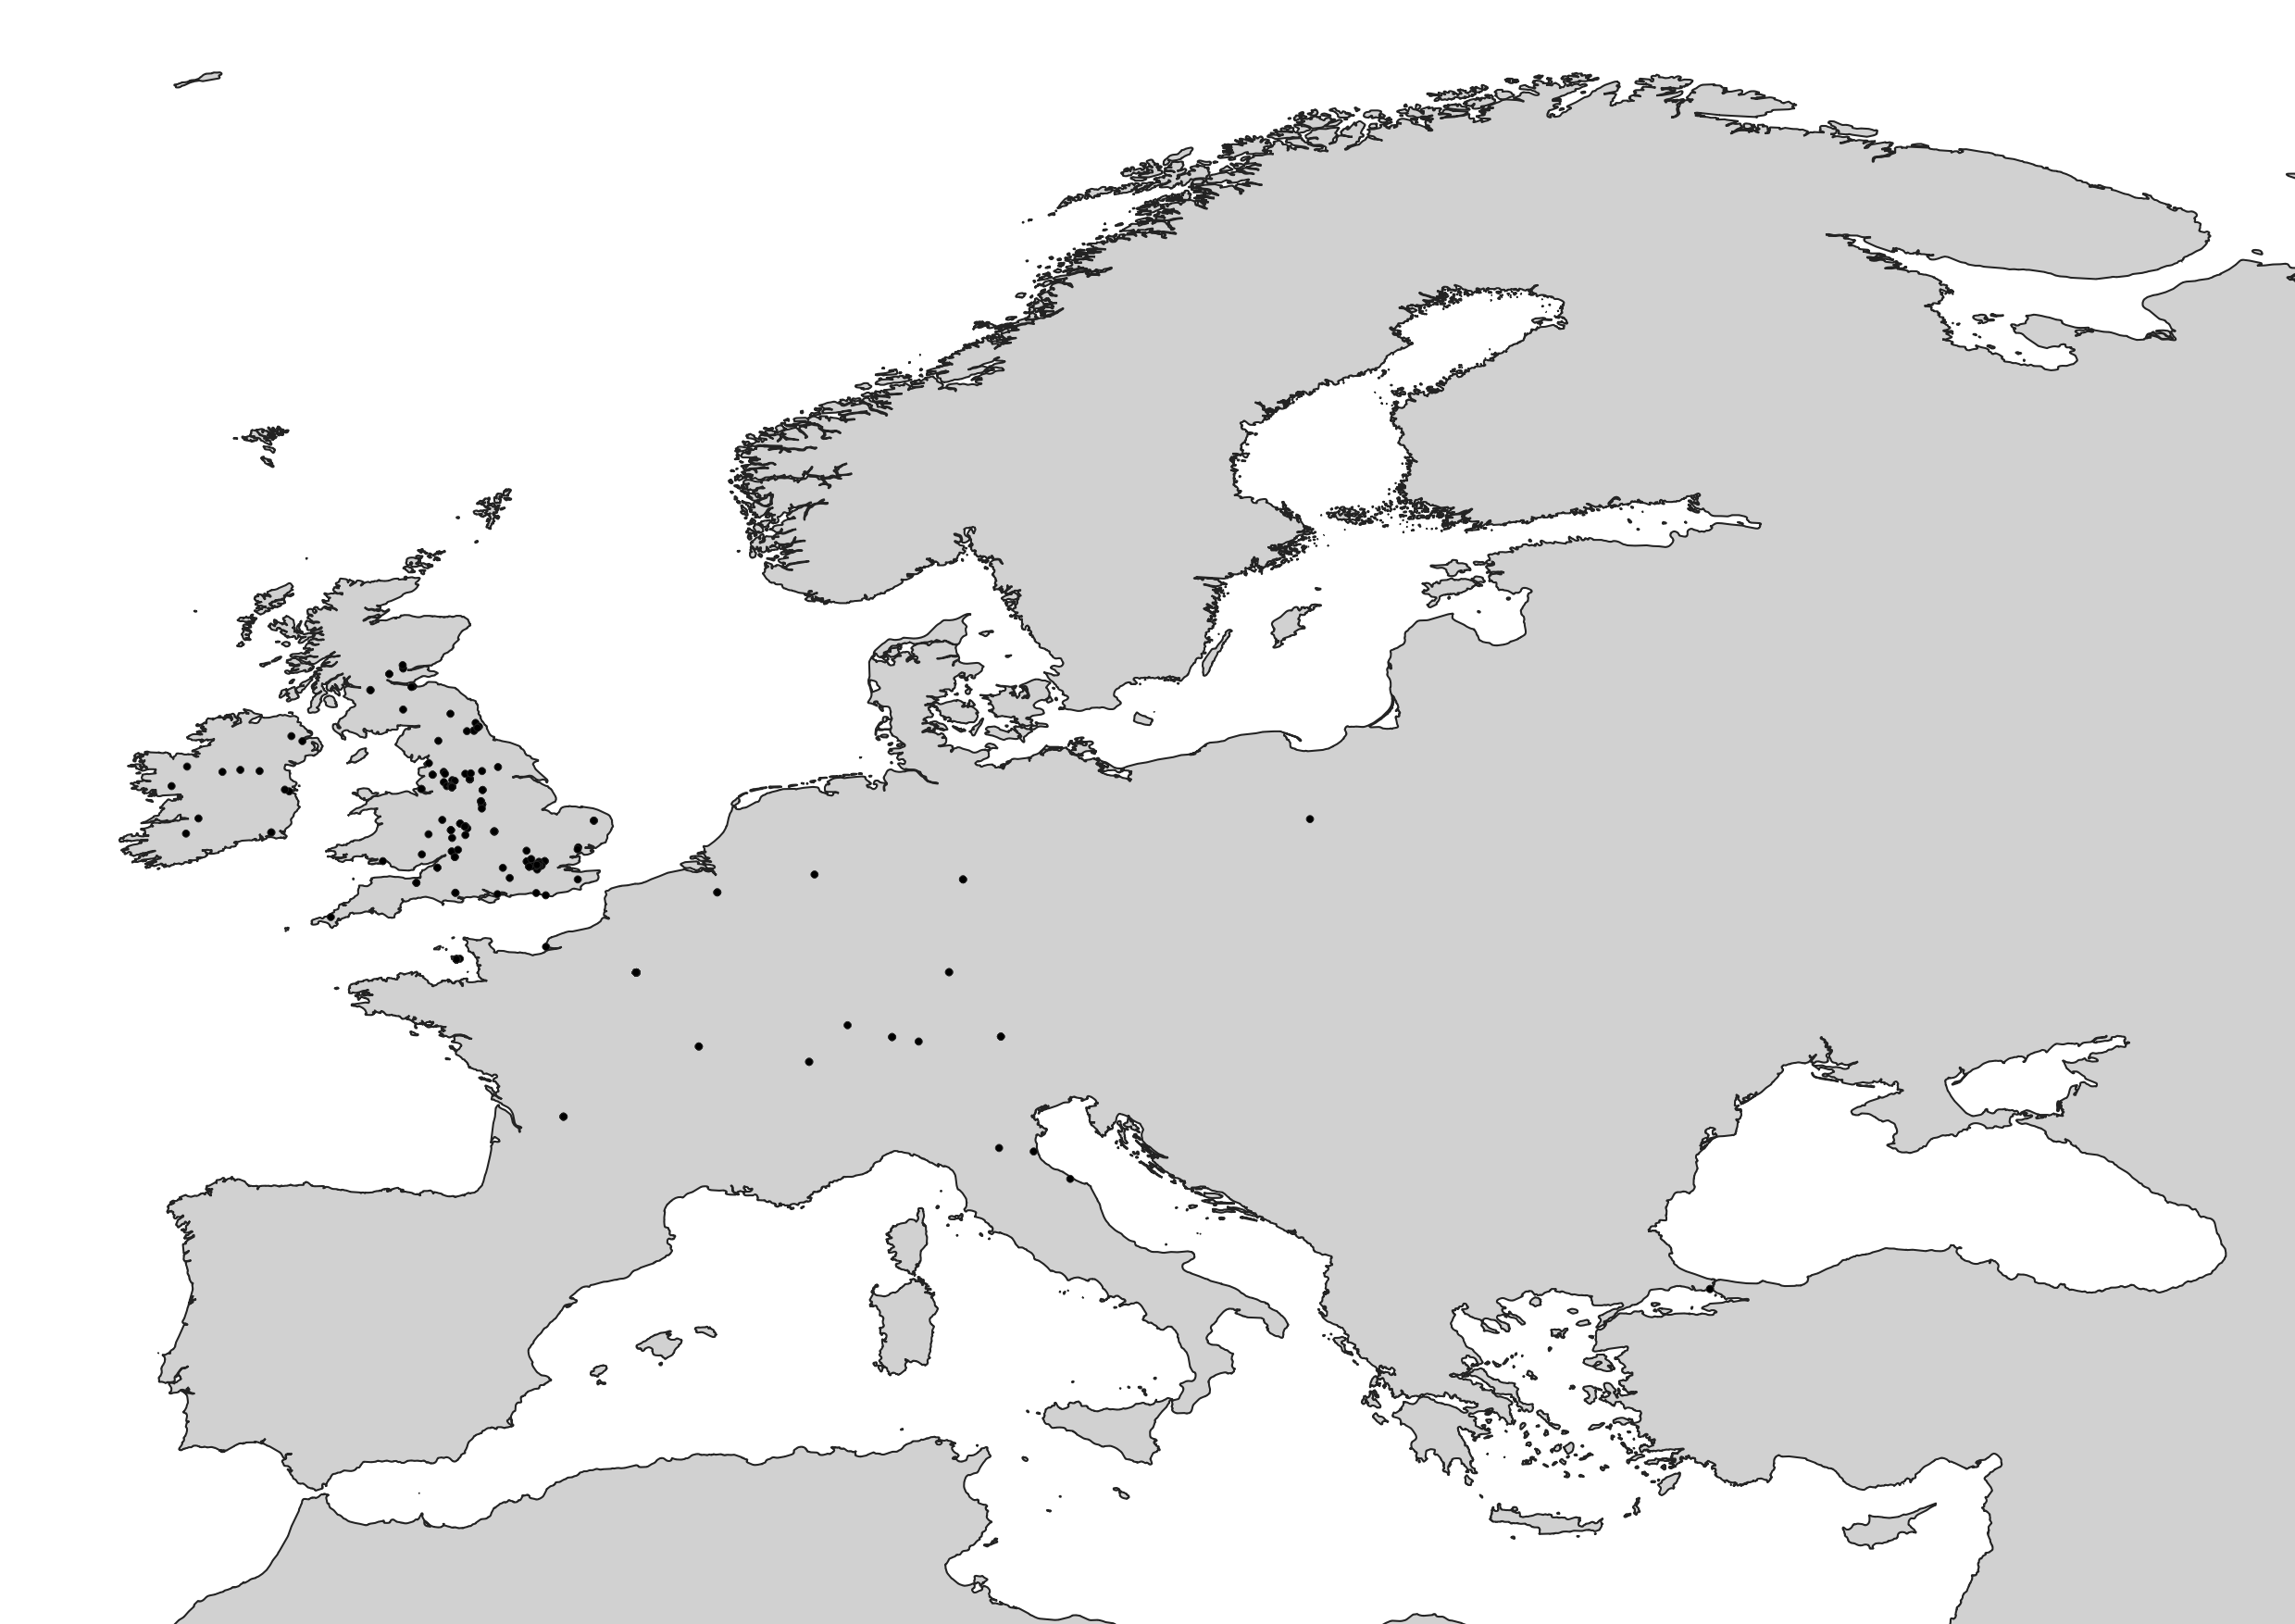
\includegraphics[width=\textwidth]{1850.png}
    \caption{1850}
    \label{fig:1850}
  \end{subfigure}
  \begin{subfigure}[b]{0.45\textwidth}
    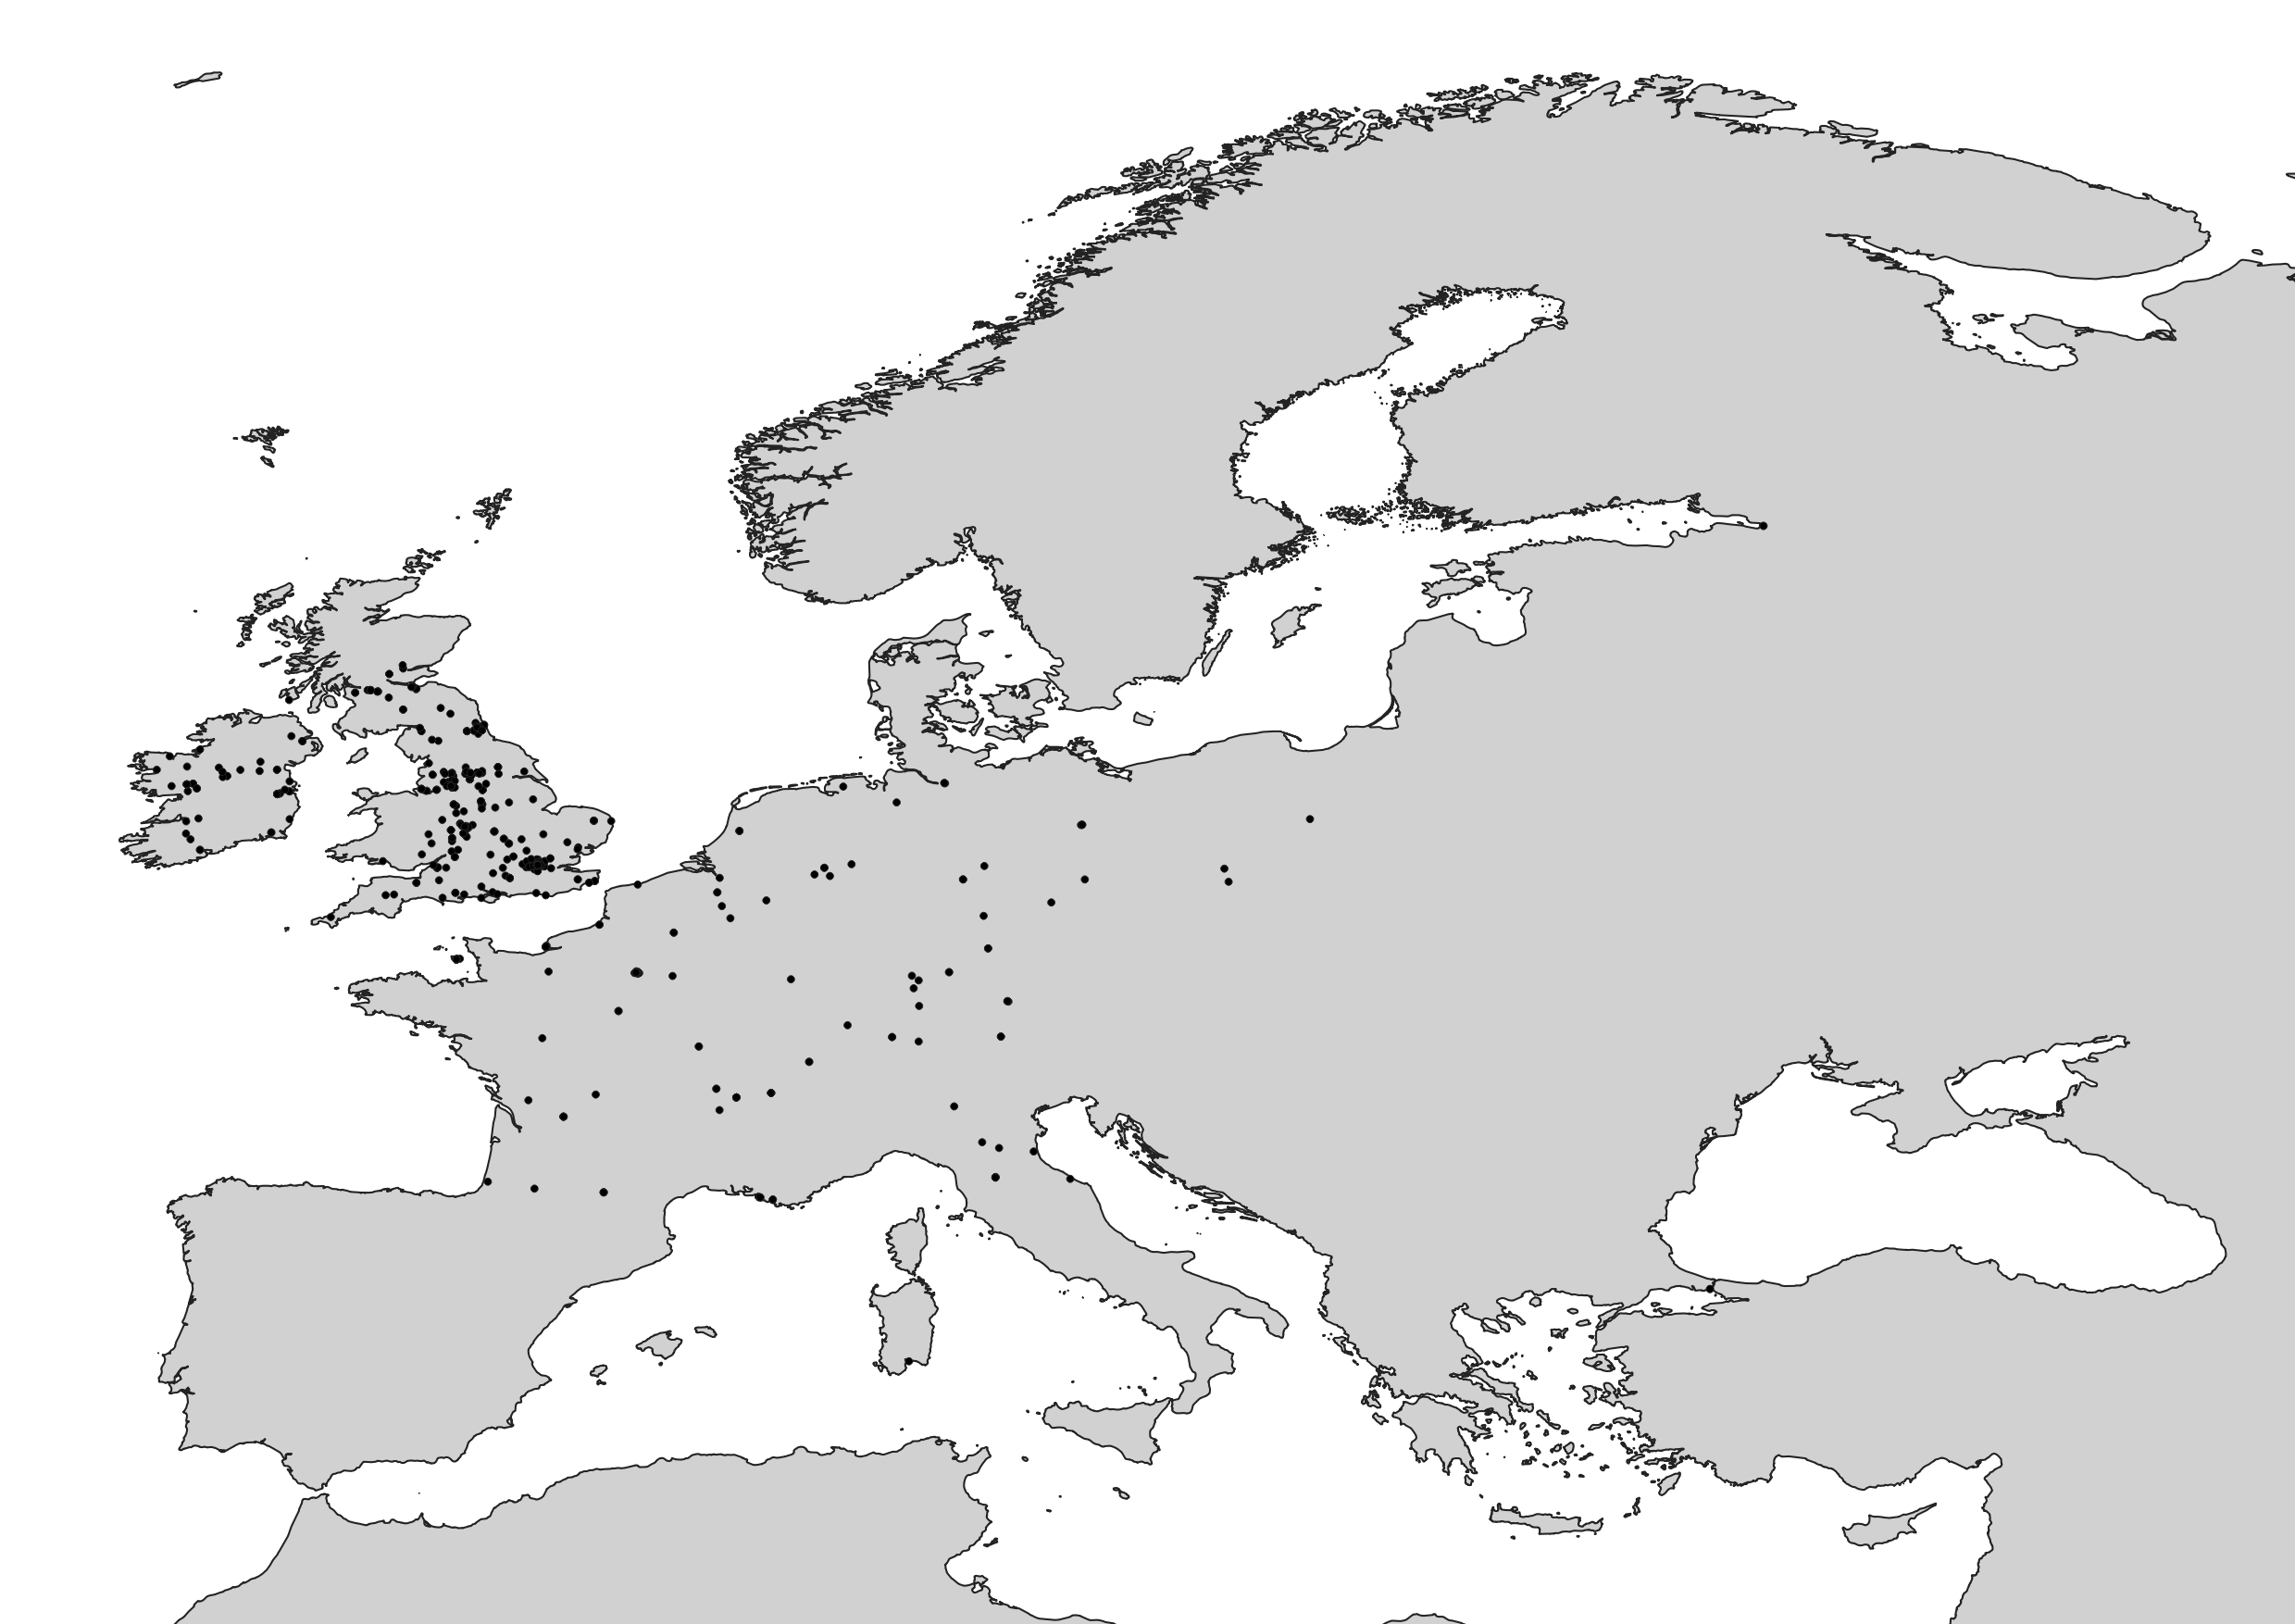
\includegraphics[width=\textwidth]{1860.png}
    \caption{1860}
    \label{fig:1860}
  \end{subfigure}

  \begin{subfigure}[b]{0.45\textwidth}
    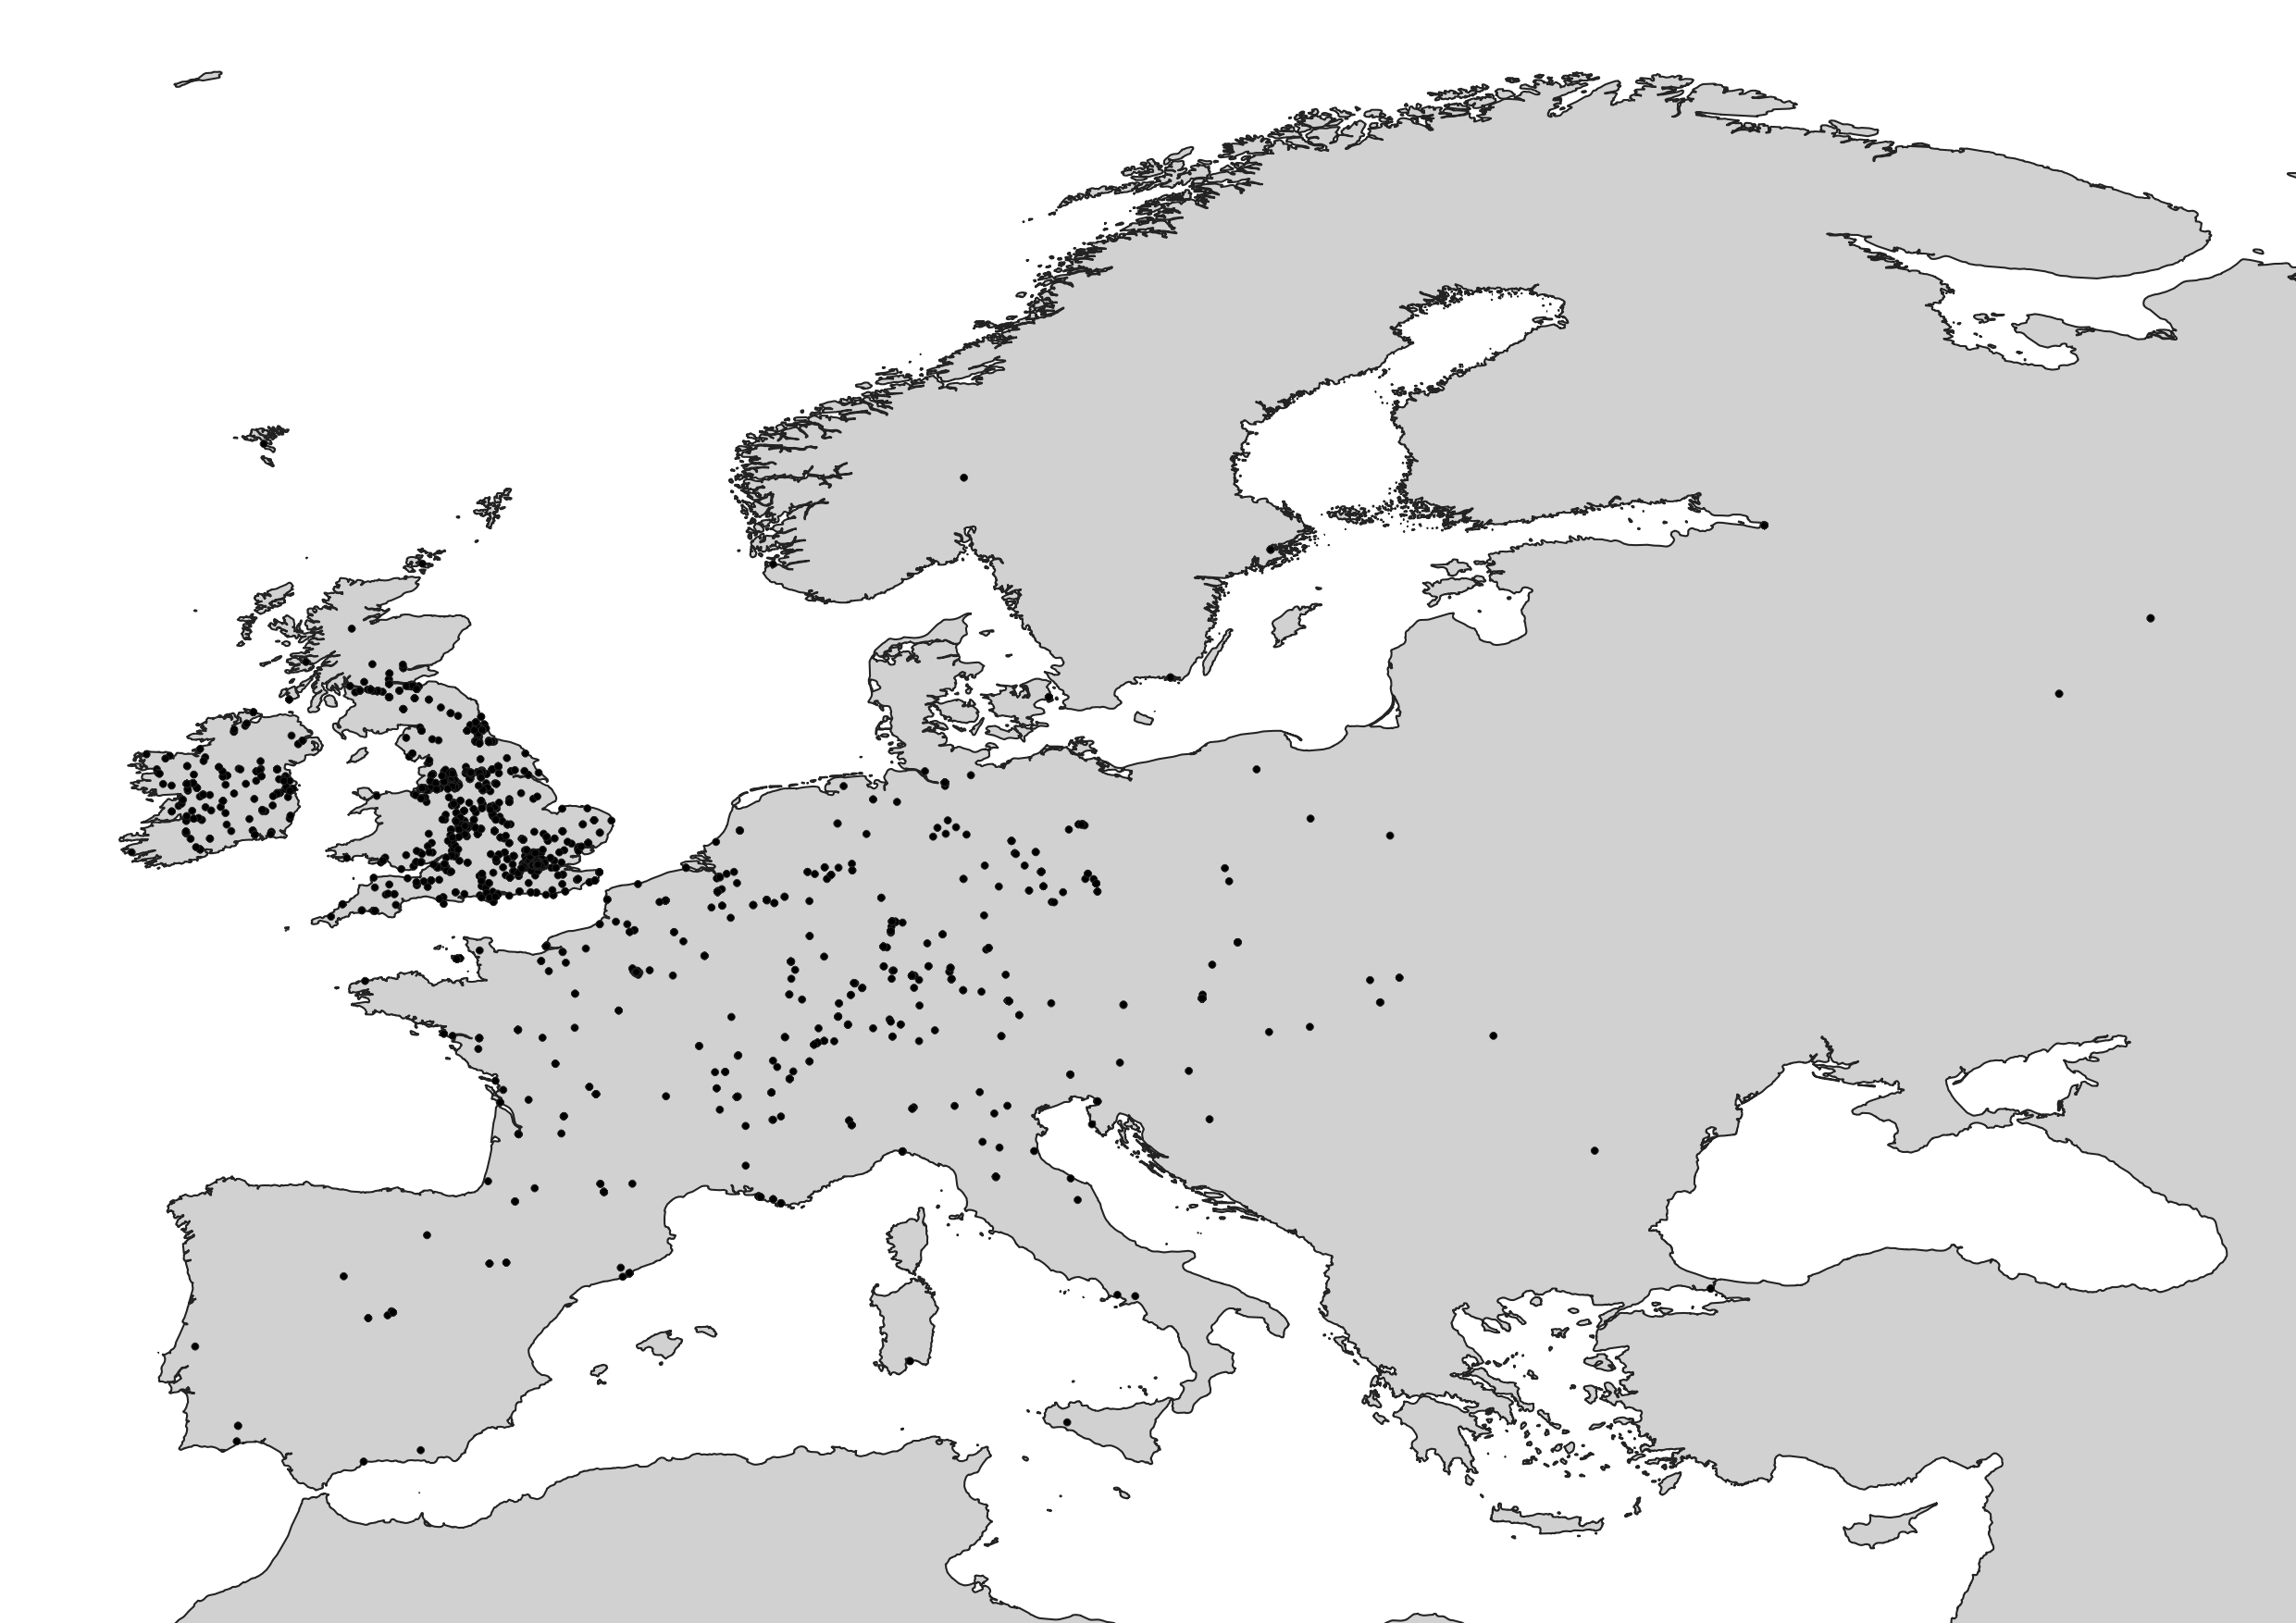
\includegraphics[width=\textwidth]{1870.png}
    \caption{1870}
    \label{fig:1870}
  \end{subfigure}
  \begin{subfigure}[b]{0.45\textwidth}
    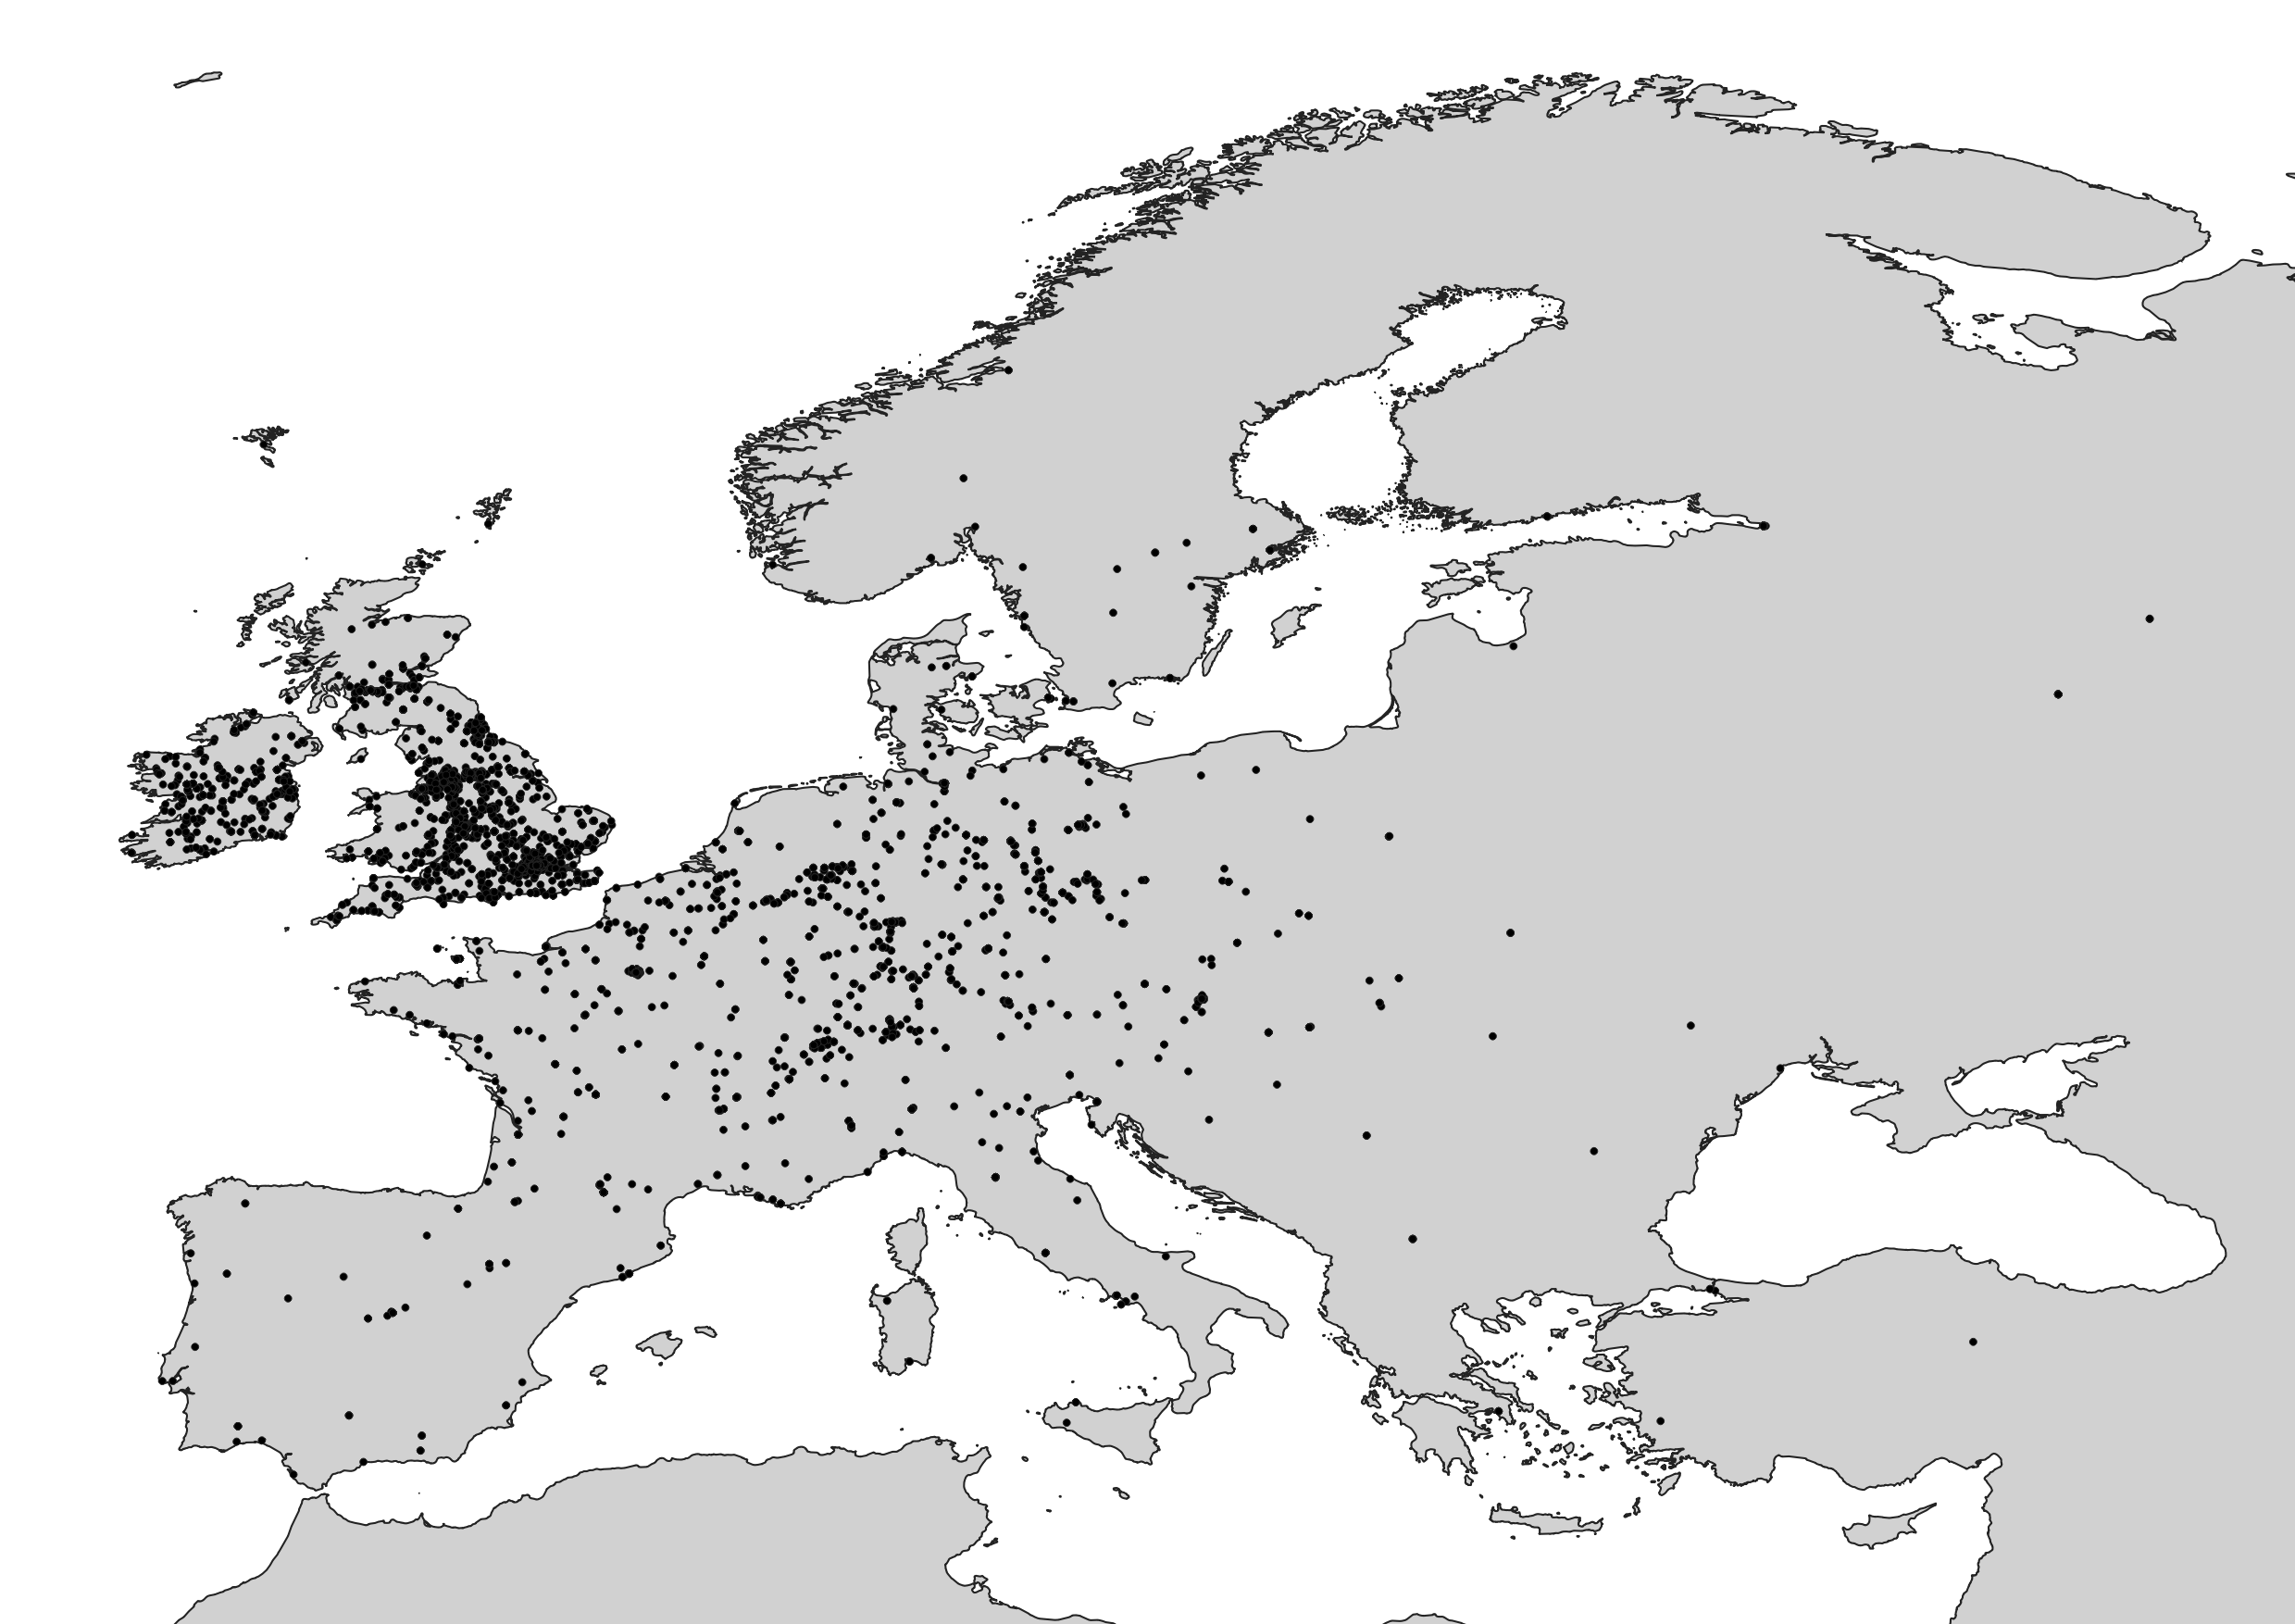
\includegraphics[width=\textwidth]{1880.png}
    \caption{1880}
    \label{fig:1880}
  \end{subfigure}

  \begin{subfigure}[b]{0.45\textwidth}
    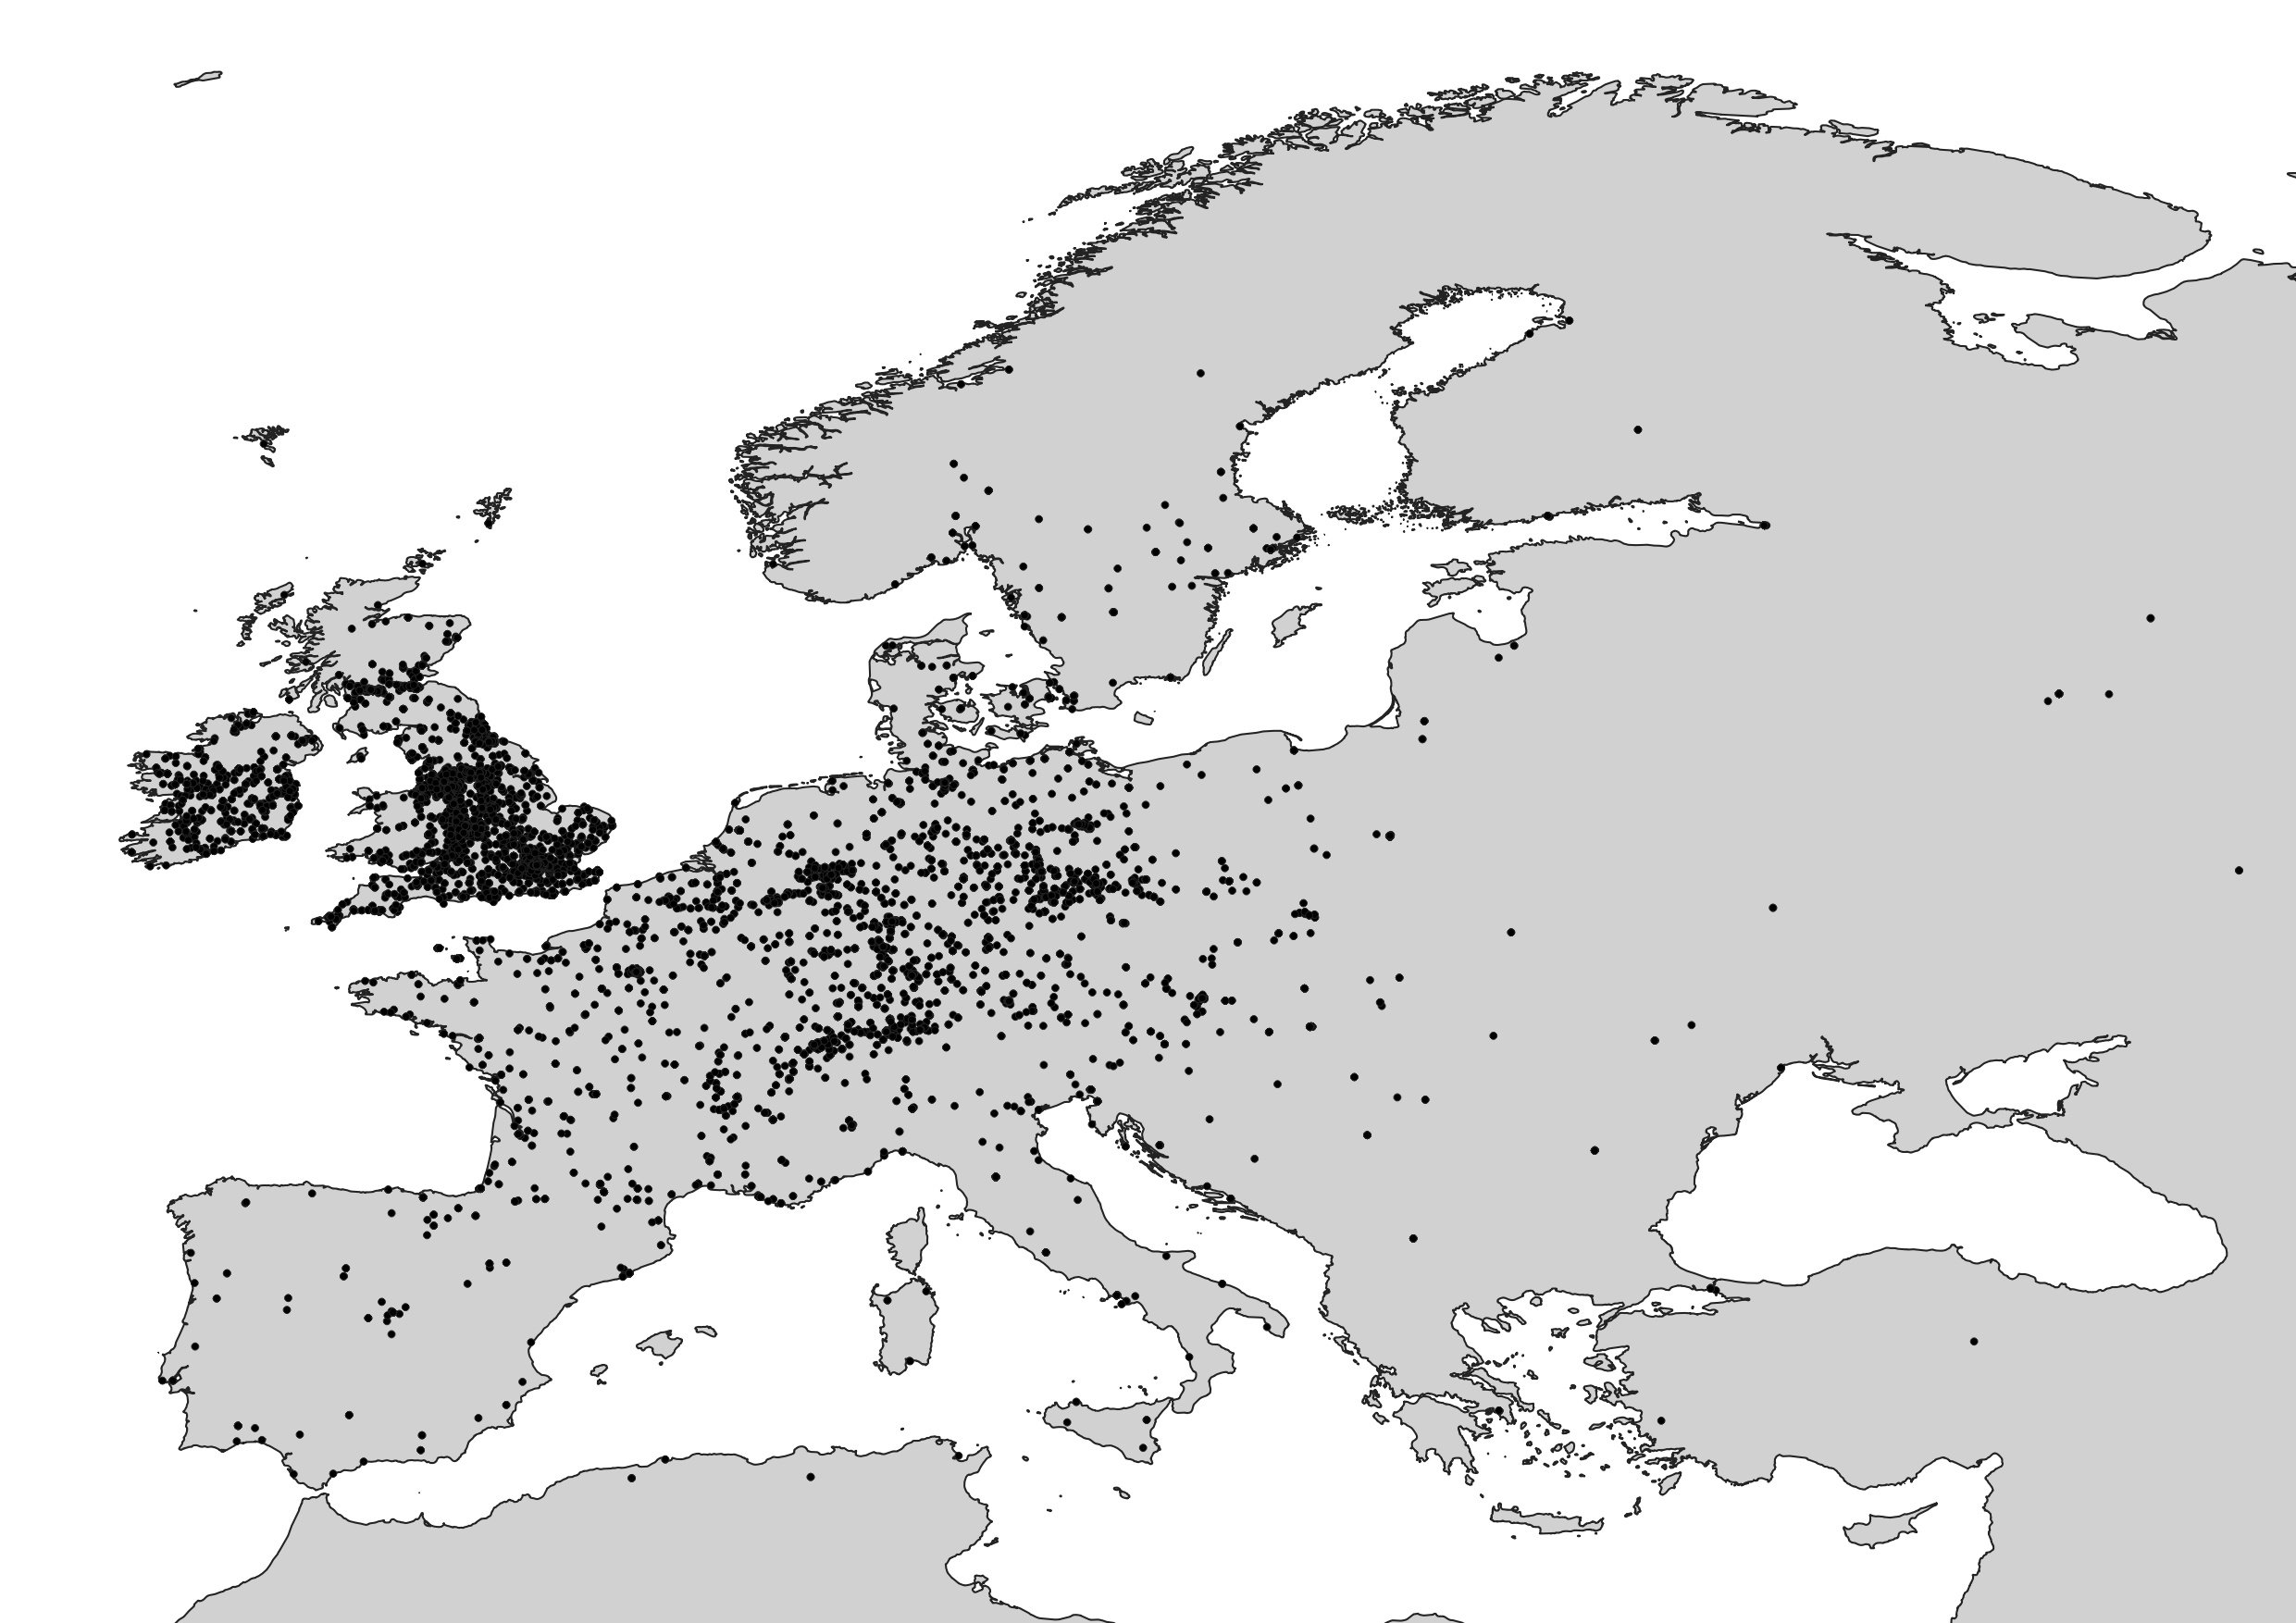
\includegraphics[width=\textwidth]{1890.png}
    \caption{1890}
    \label{fig:1890}
  \end{subfigure}
  \begin{subfigure}[b]{0.45\textwidth}
    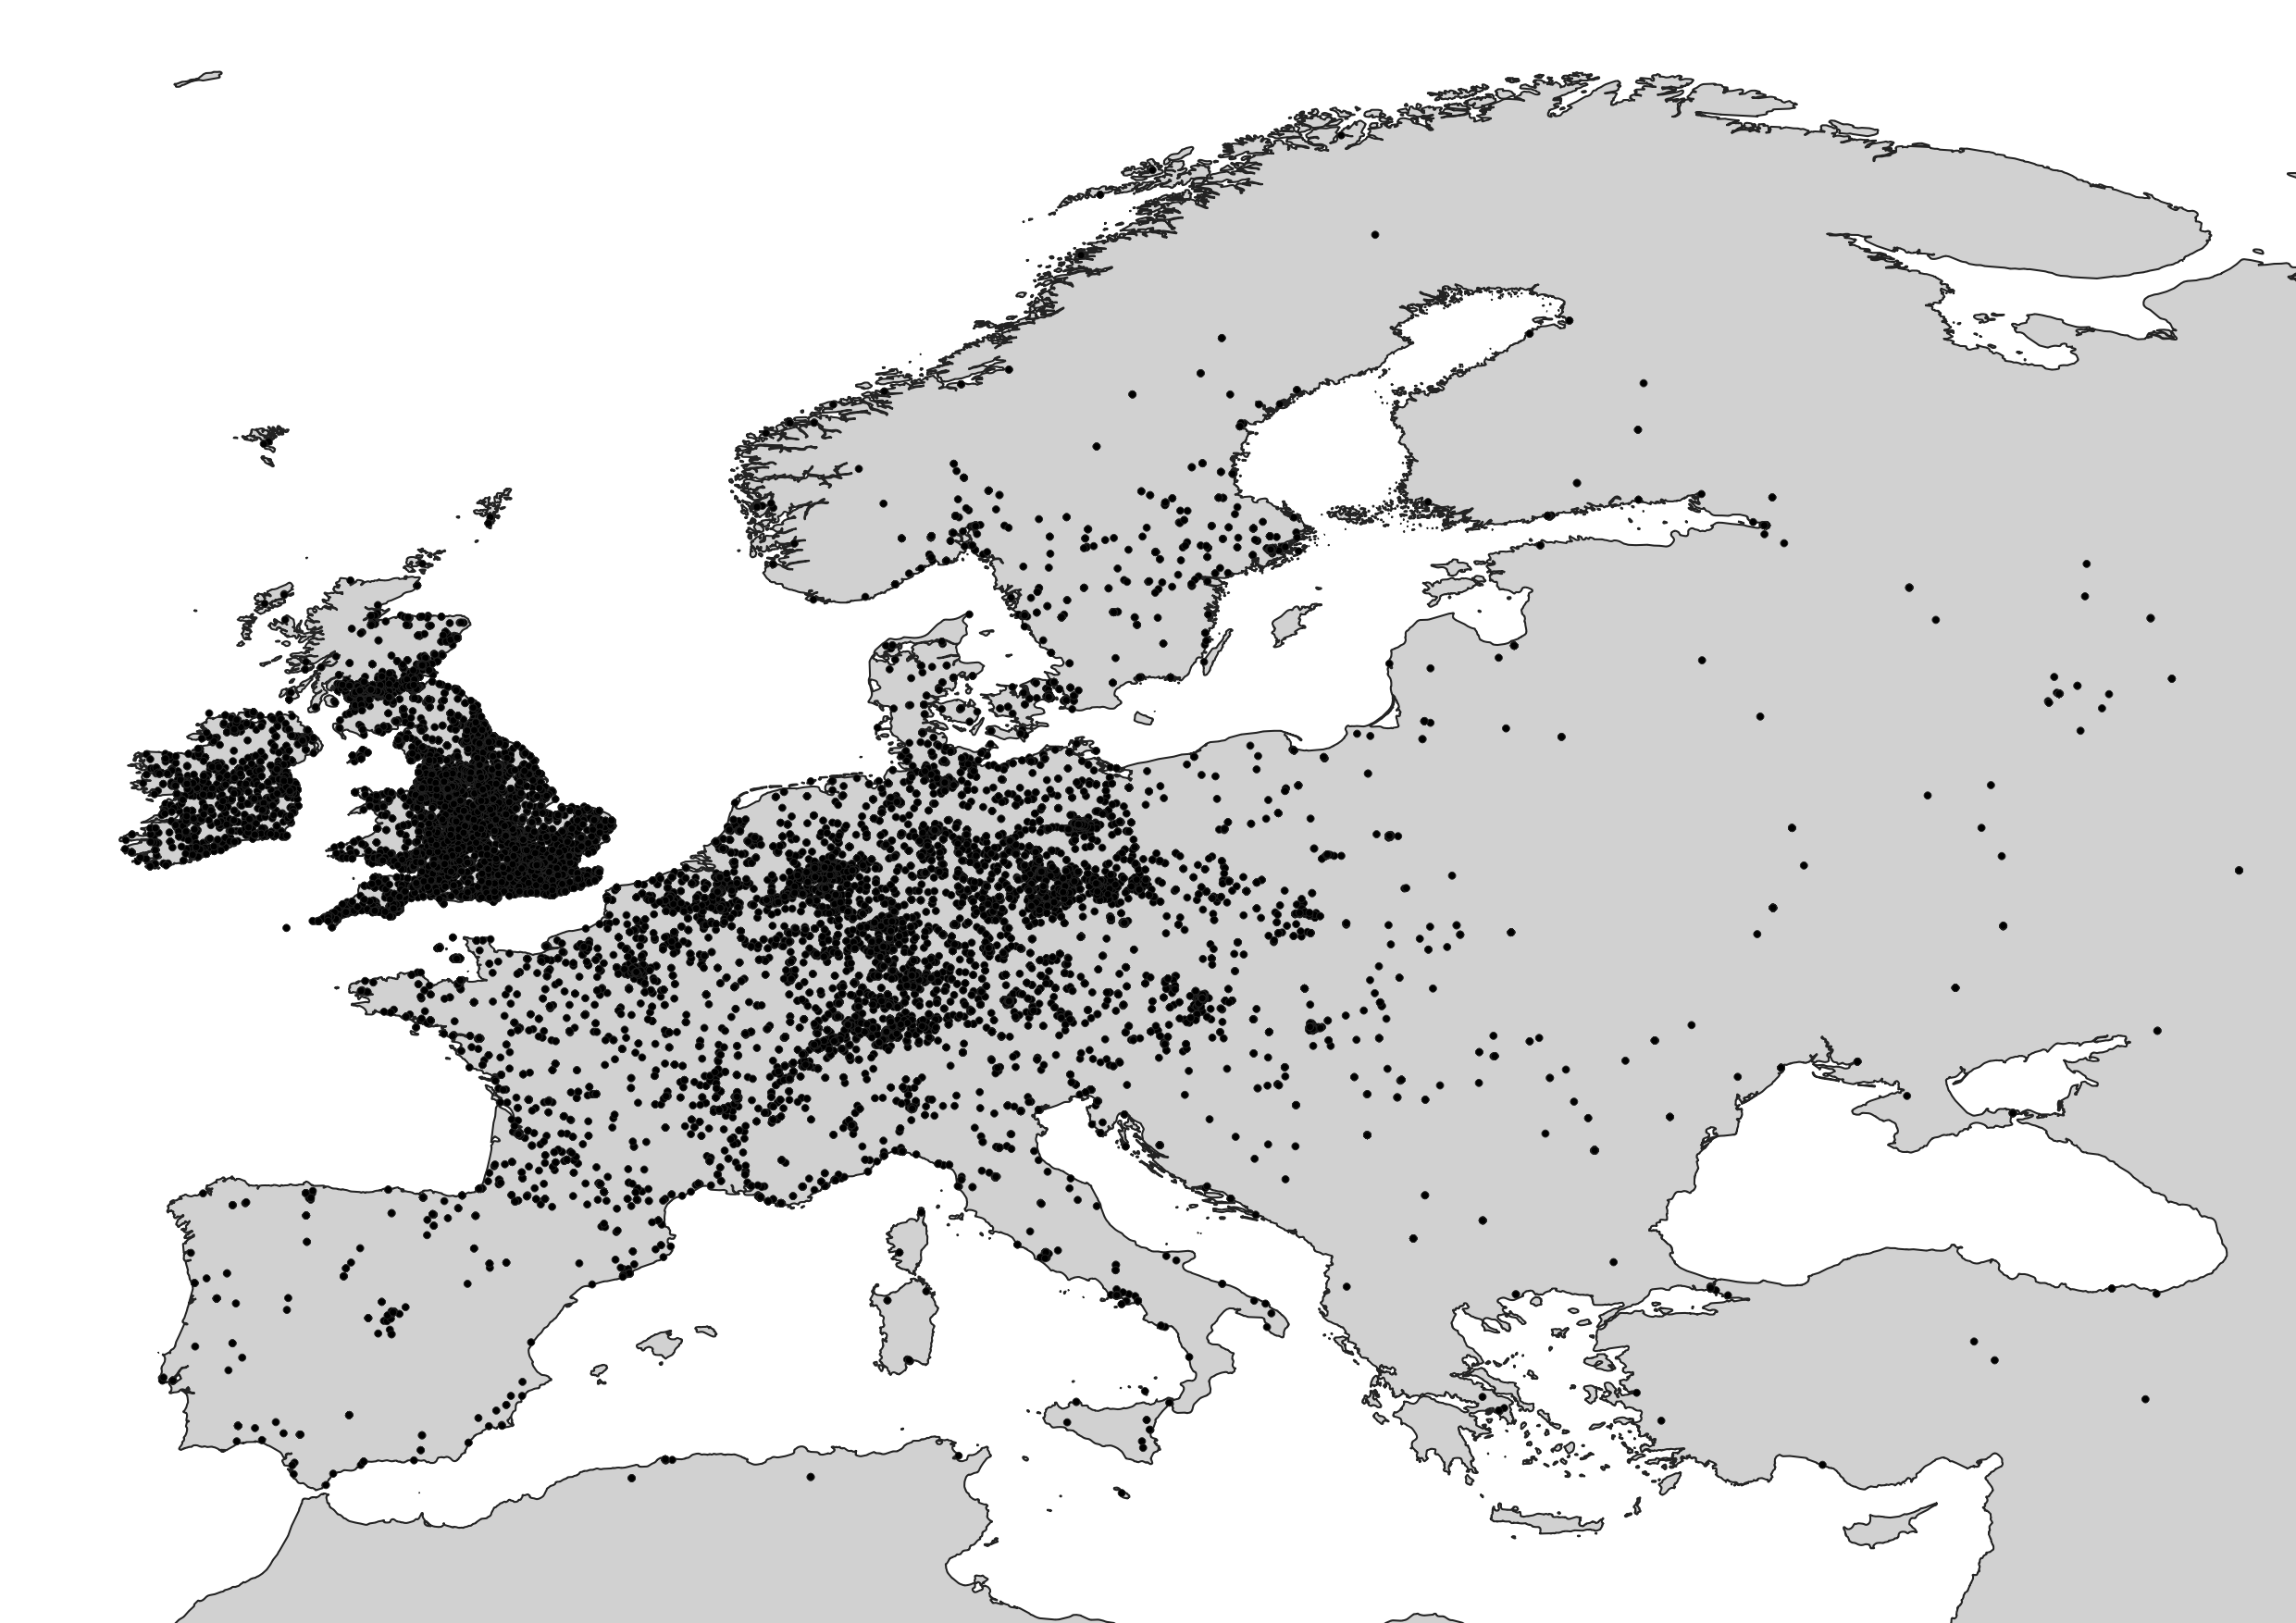
\includegraphics[width=\textwidth]{1900.png}
    \caption{1900}
    \label{fig:1900}
  \end{subfigure}

  \caption{Spatial Evolution of Patent Activity (1850-1900). Each panel displays the geographical locations of patentees who filed patents in the UK or US during the respective cumulative period (patents published before the year shown). The maps illustrate the progressive expansion of innovative activity from the core regions of Northern France and Belgium towards Southern Germany and Northern Italy.}
  \label{fig:images_1850_1900}
\end{figure}
The data reveal distinct patterns in the spatial distribution of patents. We observe early clusters of patent activity in northern France and Belgium, followed by a gradual expansion towards southern Germany and northern Italy.
Our dataset comprises more than 120 thousand patents filed by European inventors in the British and U.S. patent offices between 1835 and 1899 (i.e., published prior to 1900). The distribution of these patents across time is not uniform: patenting accelerated in the latter decades of the 19th century, likely due to both faster industrial development and changes in patenting practices and institutions.
\subsection{Directional Distribution}
To analyze the spatial distribution of patents, we employ the directional distribution method. This approach applies standard deviation calculations to two-dimensional space and can quantify directional trends in patent diffusion. The directional distribution is represented by a standard deviational ellipse, which captures the spatial spread and orientation of the data points.
The method rests on calculating spatial standard deviations:
\begin{equation}
  \scalebox{0.80}{\(\displaystyle
    \sigma_{1,2}=\left(\frac{\left(\sum_{i=1}^n \tilde{x}_i^2+\sum_{i=1}^n \tilde{y}_i^2\right) \pm \sqrt{\left(\sum_{i=1}^n \tilde{x}_i^2-\sum_{i=1}^n \tilde{y}_i^2\right)^2+4\left(\sum_{i=1}^n \tilde{x}_i \tilde{y}_i\right)^2}}{2 n}\right)^{1 / 2}
  \)}
\end{equation}
Where \(x\) and \(y\) represent the coordinates of each patent location, and the tilde values denote the difference between each coordinate and its mean. We use this to construct standard deviational ellipses (at one standard deviation) that summarize dispersion and orientation.
We applied this directional distribution analysis to each of our cumulative subgroups of patents. The results in Figure~\ref{fig:direct_distrib} reveal a clear pattern in the diffusion of patent activity across Europe during the 19th century. In each successive cumulative period, we observe a clear south-eastward elongation of the ellipses: innovation spread from northwest to southeast across the continent.
\begin{figure}
  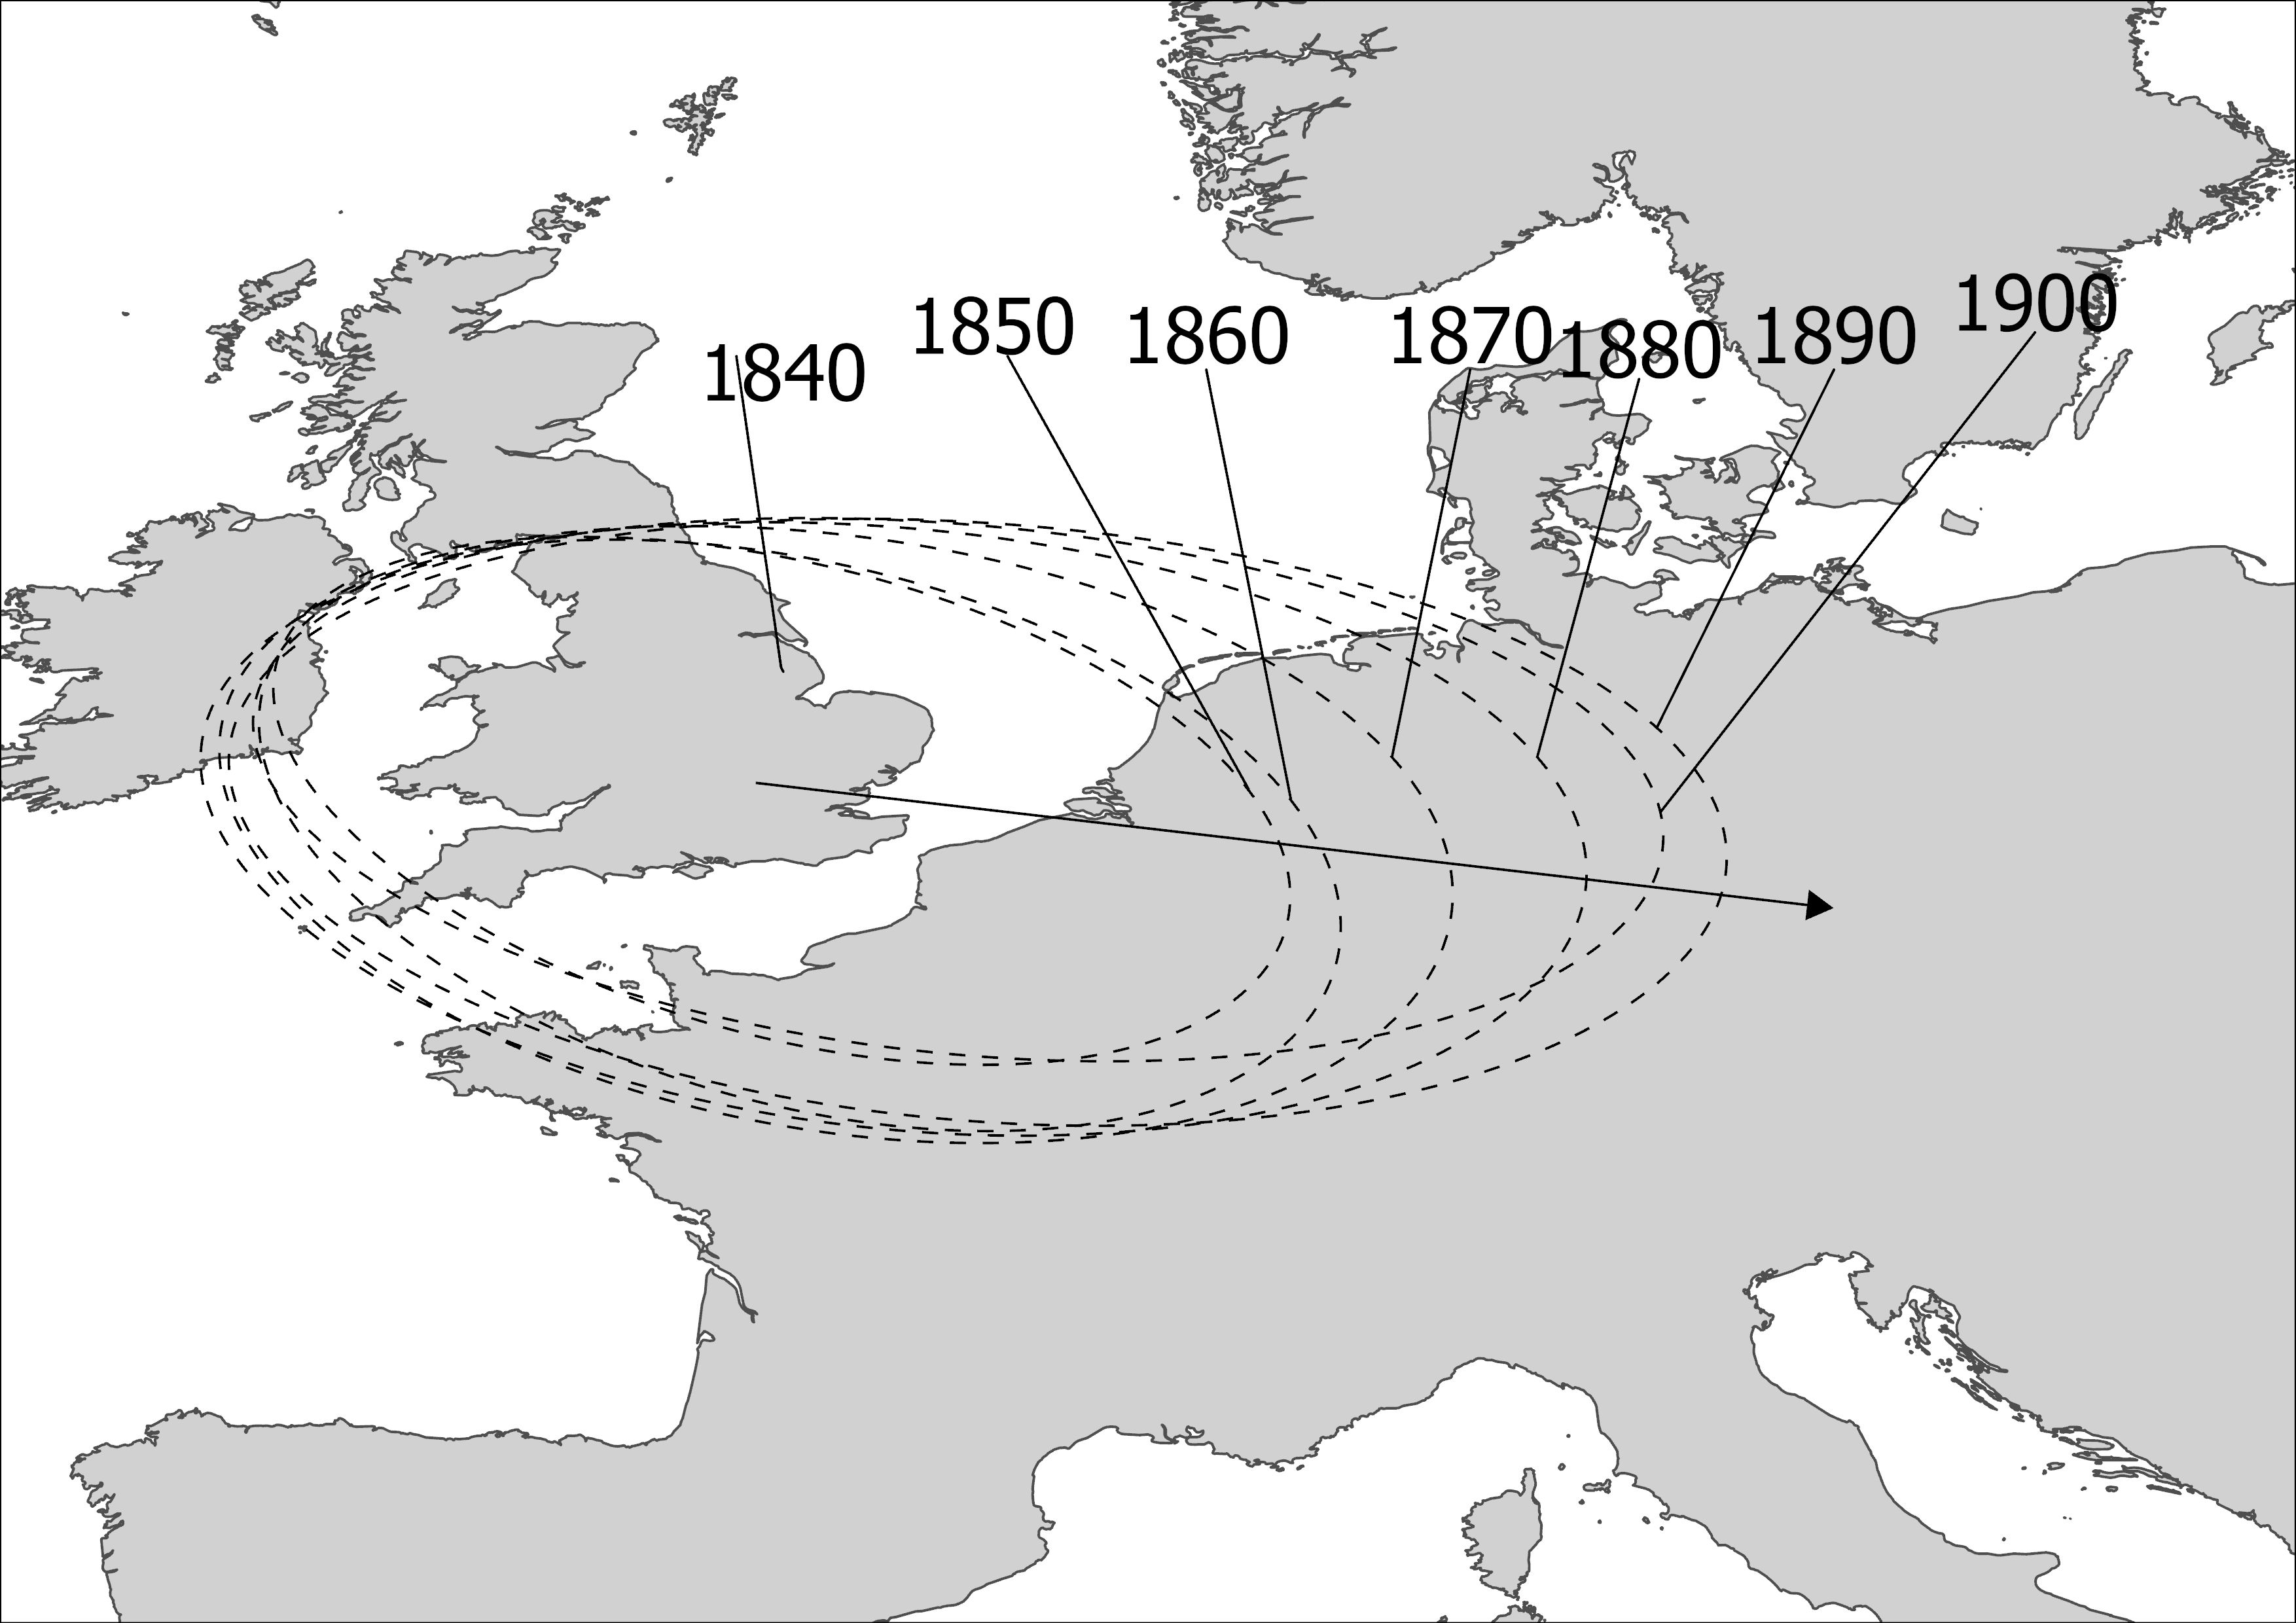
\includegraphics[width=1\linewidth]{directional_distributions.jpg}
  \caption{Directional Distribution of Patent Activity (Standard Deviational Ellipses). The ellipses summarize the directional trend of patent locations across the cumulative periods ending in 1850, 1860, \dots, 1900, computed at one standard deviation from the mean center. The elongation and rotation of the ellipses over time demonstrate a consistent south-eastward diffusion of the innovation frontier.}
  \label{fig:direct_distrib}
\end{figure}
The ellipse for the 1835-1890 group is the first to depart from this trend, reducing its south-eastward stretch. This change suggests a shift in spatial dynamics: the clear south-eastward directionality of earlier decades gave way to a more even spread across the continent.
The directional trajectory overlaps suggestively with the urban-industrial corridor later conceptualized as the ``Blue Banana'' \citep{brunet1989lieues}, a discontinuous arc of urbanization stretching from Northwest England to Northern Italy. 
\subsection{Spatiotemporal Diffusion Patterns}
\label{sec:kde}
To characterize the spatiotemporal evolution of patent activity across Europe, we adapt the standard kernel density estimation (KDE) framework by incorporating a temporal component with cumulative time windows. This adaptation lets us document the spatial and temporal dimensions of the innovation diffusion process simultaneously, through density surfaces that show how patent activity spread across the continent over time.
The standard kernel density estimation is a non-parametric method for estimating probability density functions. In spatial analysis, KDE interpolates the density of point patterns across a continuous surface. We adapt this method to our historical context, using patent locations as point data to estimate the intensity of innovative activity across Europe.
The standard KDE formulation at location \(i\) with a quartic kernel is expressed as:
\begin{equation*}
  \begin{aligned}
    KDE_i &= \frac{1}{b^2} \sum_{j=1}^n \left[\frac{3}{\pi} \cdot A_j \left(1-\left(\frac{\delta_{ij}}{b}\right)^2\right)^2\right], \\
    &\quad \text{for } \delta_{ij} < b
  \end{aligned}
\end{equation*}
Where:
\begin{itemize}
  \item \(b\) is the bandwidth or search radius
  \item \(A_j\) is a weight associated with observation \(j\)
  \item \(\delta_{ij}\) is the Euclidean distance between location \(i\) and observation \(j\)
  \item \(n\) is the total number of observations
\end{itemize}
Note that the condition \(\delta_{ij} < b\) ensures that only observations within the bandwidth contribute to the density estimation.

To incorporate the temporal dimension of the diffusion process, we modify the formulation to include time and condition the estimation on cumulative time windows. The modified equation becomes:
\begin{equation}
  \label{eq:spatiotemporal}
  \begin{aligned}
    KDE_{i,t}(t \leq T) &= \frac{1}{b^2} \sum_{j=1}^n \left[\frac{3}{\pi} \cdot A_j \cdot I(t_j \leq T) \left(1-\left(\frac{\delta_{ij}}{b}\right)^2\right)^2\right], \\
    &\quad \text{for } \delta_{ij} < b
  \end{aligned}
\end{equation}
Where:

\begin{itemize}
  \item \(t\) represents the current time point
  \item \(T\) is the upper bound of the cumulative time window
  \item \(I(t_j \leq T)\) is an indicator function that equals 1 if the time of observation \(j\) (\(t_j\)) is less than or equal to \(T\), and 0 otherwise
\end{itemize}

This formulation estimates the kernel density at location \(i\) and time \(t\) using only observations up to time \(T\). By varying \(T\), we can create moving cumulative time windows to analyze the diffusion of patenting activity over time.
The application of this model to our dataset yields a matrix of location densities across the European space. This approach has two practical advantages for studying historical industrialization. First, it interpolates point data over a continuum of space without relying on predetermined administrative boundaries, useful for 19th-century Europe, where borders frequently changed. Second, the method computes densities within a constant area size, which makes comparisons between regions with varying local administrative divisions more reliable.
We set the bandwidth to \(b = 250\)~km and evaluate the KDE at each NUTS2 centroid using an EPSG:3035 equal-area projection. To determine the patenting intensity threshold, we compute the 75th percentile of the cross-sectional distribution of positive KDE densities in 1850, the earliest decade in which a substantial number of regions exhibit non-zero patenting activity. A region is classified as having crossed the patenting intensity threshold, which we interpret as a proxy for industrial take-off, in the first decade in which its KDE density exceeds this value. Figure~\ref{fig:diffusion_waves} shows the resulting diffusion waves across Europe and how high-density patent areas expanded over time.
\begin{figure}
  \centering
  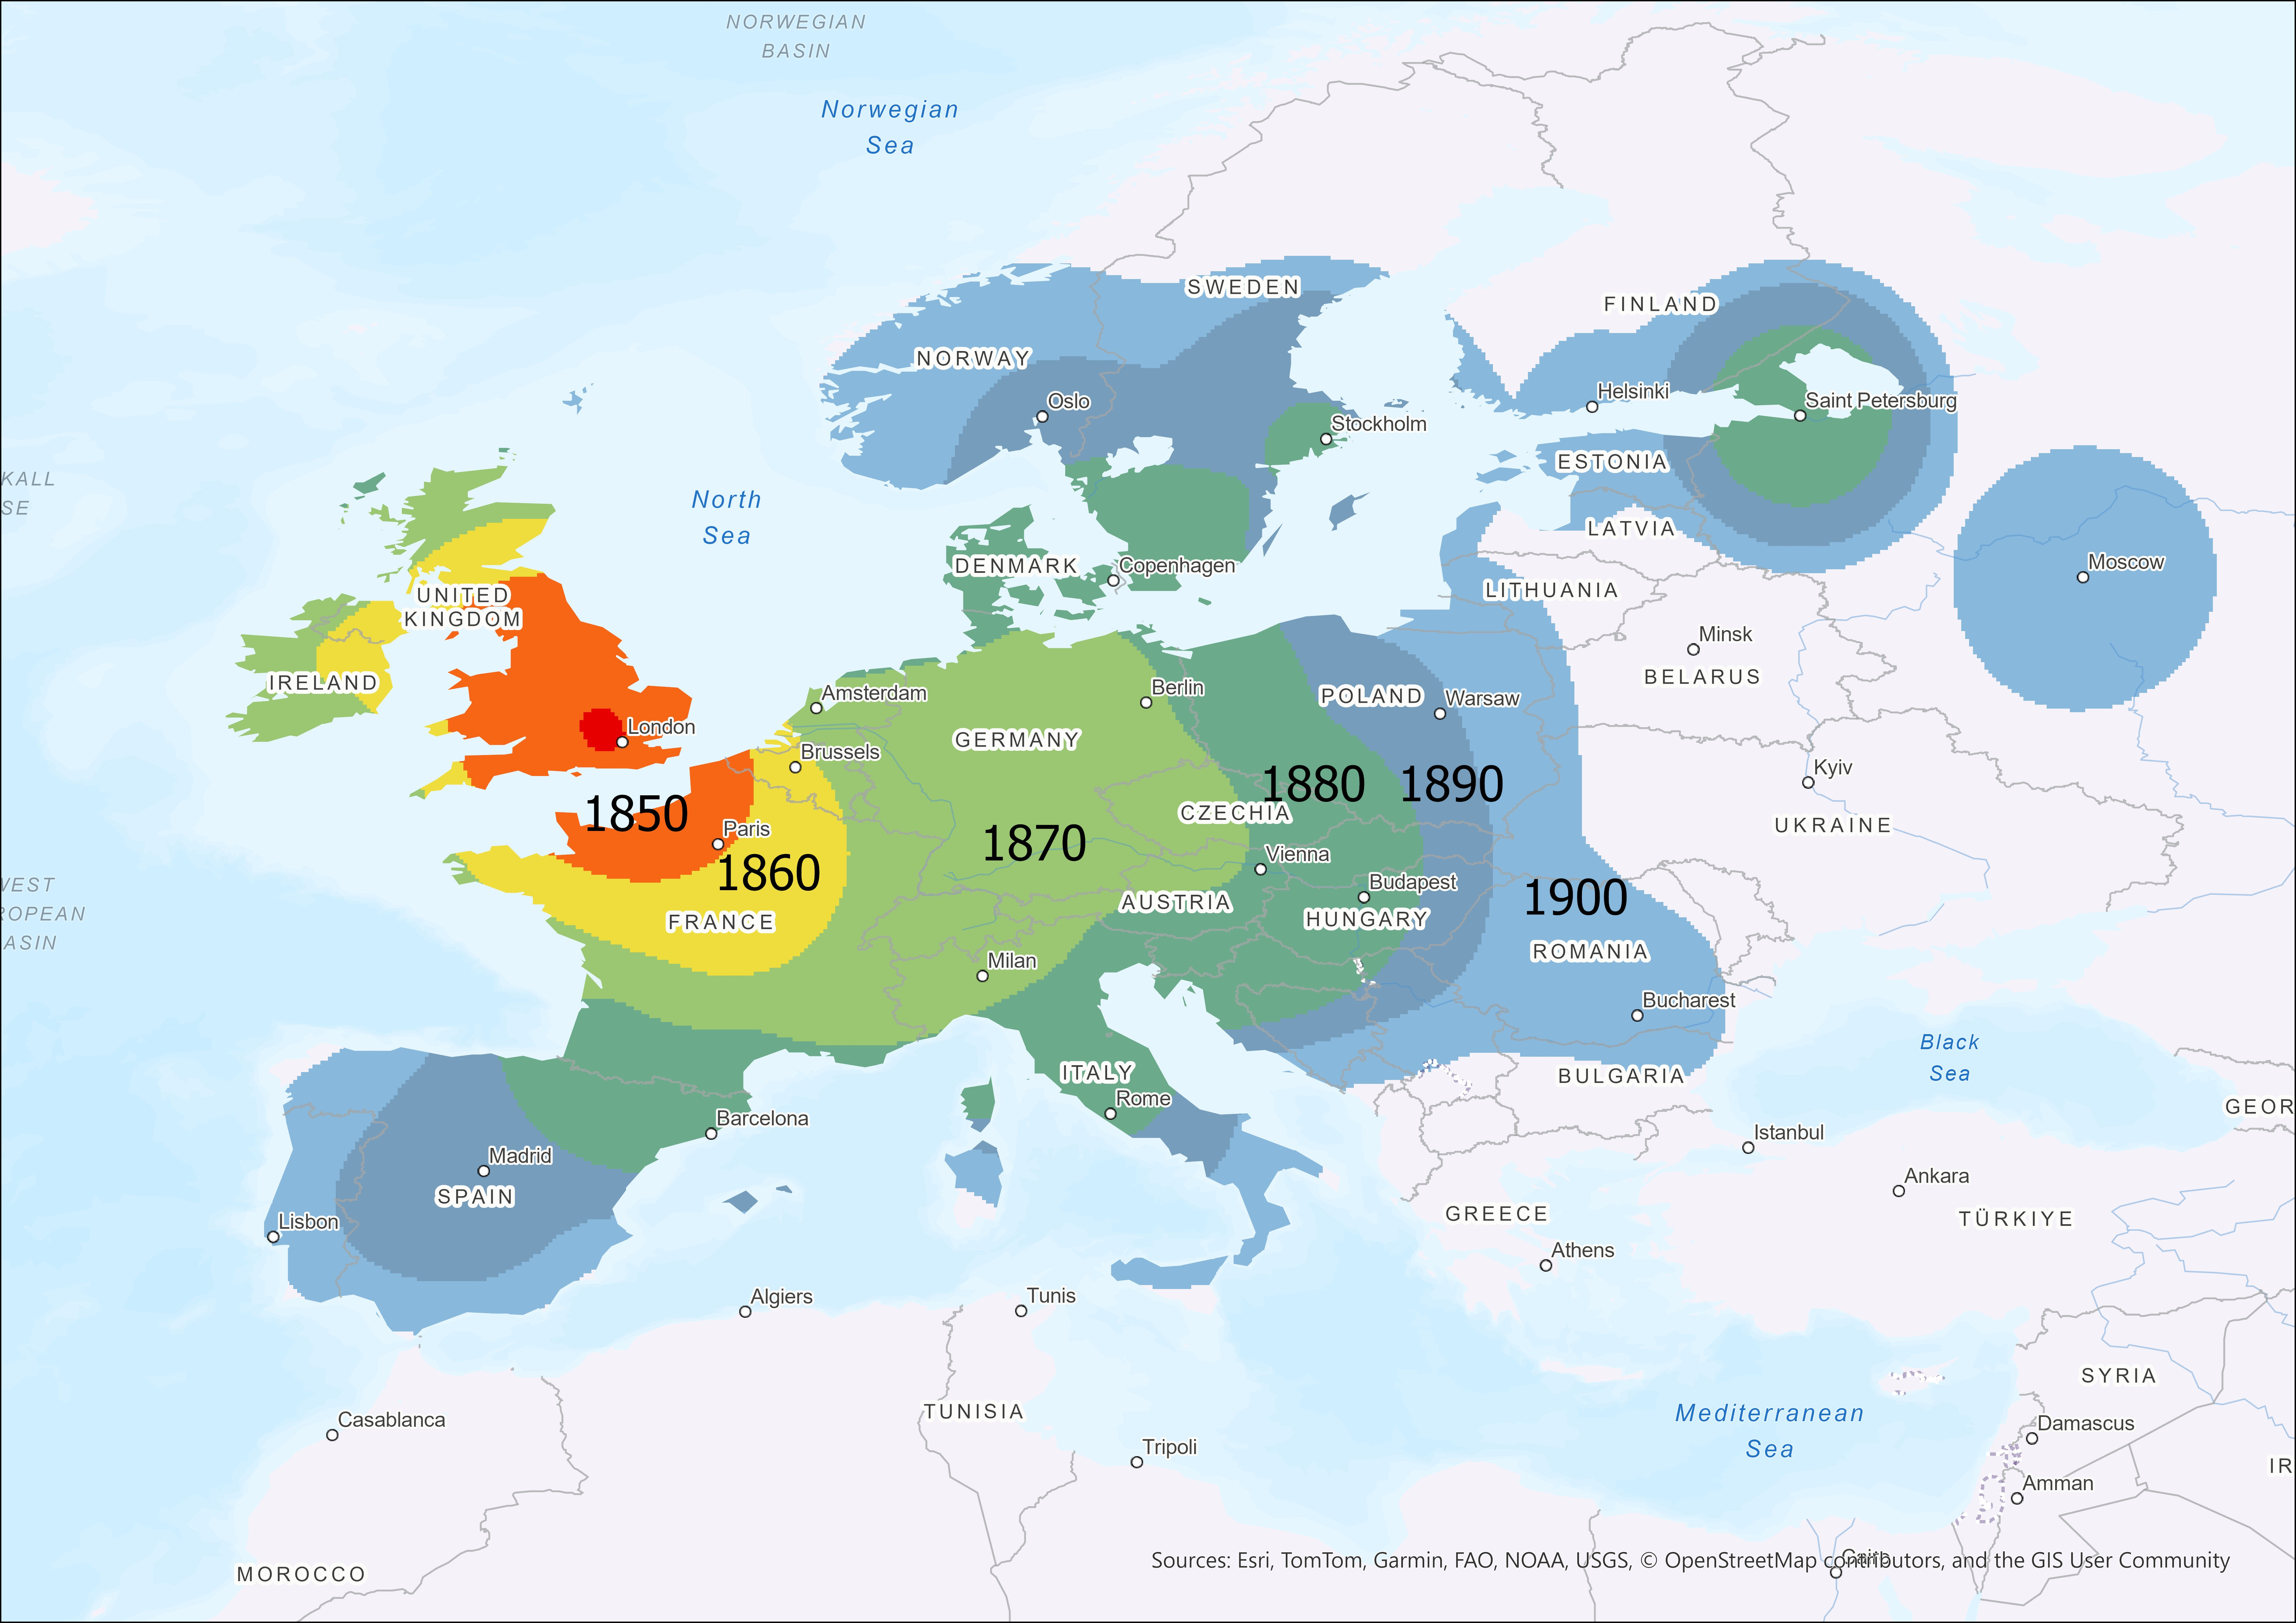
\includegraphics[width=1\linewidth]{pat_diffusion.jpg}
  \caption{Identification of Patenting Diffusion Waves. The map visualizes the spatial diffusion of inventive activity defined by patent density thresholds; these waves are interpreted as a proxy for the timing of industrial take-off. Regions are classified based on the decade they first crossed the specified patent density threshold; the resulting pattern shows wave-like propagation originating from the industrial core.}
  \label{fig:diffusion_waves}
\end{figure}
This approach yields a proxy variable for industrialization at the regional level. Regions that never cross the KDE threshold by 1899 are treated as right-censored at 1900. The resulting event definition provides the dependent variable for the Cox proportional hazards model estimated in Section~\ref{sec:cox}.

The diffusion waves in Figure~\ref{fig:diffusion_waves} reveal a clear, spatially dependent pattern of innovation spread: activity originates near the British epicenter and radiates outward with a pronounced south-eastward drift. These stylized facts raise a natural question: what mechanisms drive this wave-like diffusion? In the following section, we develop a gravity-based model of knowledge spillovers to provide a structural explanation for the patterns documented here.

\subsection{Descriptive Statistics}

Table~\ref{tab:descriptive} presents summary statistics for the main variables used in our econometric analysis. The dataset covers European NUTS2 regions over the decade endpoints 1840--1900 (patents published prior to 1900).

\begin{table}[!htbp]
\centering
\caption{Descriptive Statistics}
\label{tab:descriptive}
\footnotesize
\begin{tabular}{lrrrrr}
\toprule
Variable & Mean & SD & Min & Max & N \\
\midrule
Patents (count) & 12.83 & 74.56 & 0.00 & 1,806.00 & 2,023 \\
Patent Stock (count) & 22.13 & 143.89 & 0.00 & 4,231.00 & 2,023 \\
Population (thousands) & 173.81 & 270.24 & 1.00 & 2,953.00 & 2,023 \\
Spillover Index (billions) & 839.96 & 31,983.24 & 0.00 & 1,425,912.21 & 2,023 \\
Coal Cost (index) & 96.63 & 74.07 & 3.17 & 402.42 & 2,023 \\
Distance from London (km) & 1,182.74 & 564.39 & 228.20 & 3,217.55 & 2,023 \\
\bottomrule
\end{tabular}
\end{table}


\section{Model and Estimation}
We construct a parsimonious econometric model that draws on the gravity trade literature.
The underlying idea is that, similarly to trade, idea flows between two locations depend positively on the population size of each location and negatively on the communication cost between them. We argue that this mechanism can explain the European industrialization waves observed in the data, and in particular the ``nearby-diffusion'' and ``jump'' diffusion dynamics discussed above.

One of the main challenges of studying economic history is the scarcity of high-resolution data. We do not have data on bilateral trade flows or migration among regions at the subnational level. The model's parsimony reflects both the complexity of the phenomenon and the constraints of the available data.
\subsection{The model}
\subsubsection*{The flow of ideas}
Consider a geography composed of \(N\) locations, denoted by subscripts. Time is discrete, and at time \(t\), two locations \(i\) and \(j\) communicate following the gravitational approach.
\begin{equation}
  \label{eq:connection}
  C_{ij,t}=G\cdot\frac{{Pop}_{i,t}^\alpha   \cdot   Pop_{j,t}^\beta}{T_{ij,t}},
\end{equation}
where
\begin{itemize}
  \item \(C_{ij,t}\) is the communication intensity between locations \(i\) and \(j\) at time \(t\)
  \item \(Pop_{i,t}\) and \(Pop_{j,t}\) are the respective populations of location \(i\) and \(j\) at time \(t\)
  \item \(T_{ij,t}\) is the bilateral communication cost between the two locations at time \(t\)
  \item \(G\), \(\alpha\), and \(\beta\) are parameters
\end{itemize}
Each period, individuals contribute to the industrial knowledge of their location, which depends on previous cumulated knowledge, current population, and ideas arriving from other locations through bilateral connections.
\subsubsection*{The knowledge generation process}
Formally, the industrial knowledge of location \(i\) in each period is a function of past cumulated knowledge, current population, knowledge received through interactions with other locations, and technological input prices.
\begin{equation}
  \label{eq:knowledge}
  ik_{i,t} = IK_{i,t-1}^\gamma Pop_{i,t}^\eta \left( \sum_{j\neq i}C_{ij,t}IK_{j,t-1}\right)^\varepsilon \cdot IP^{-\theta}
\end{equation}
\begin{itemize}
  \item \(ik_{i,t}\) is the industrial knowledge of location \(i\) at time \(t\)
  \item \(IK_{i,t-1}\) is the cumulated industrial knowledge of location \(i\) until the previous period
  \item \(\sum_{j\neq i} C_{ij,t} IK_{j,t-1}\) is the knowledge gained from interactions with other locations
  \item \(IP\) is the input price index
  \item \(\gamma\), \(\eta\), \(\varepsilon\), and \(\theta\) are parameters
\end{itemize}
The interaction component is stronger for nearby and populated locations than for small and distant ones, a parsimonious formulation of spatial spillovers that can account for the diffusion patterns observed in the data.

Substituting equation~\eqref{eq:connection} into~\eqref{eq:knowledge}, we obtain a single knowledge creation function:
\begin{equation}
  \label{eq:final}
  ik_{i,t} = IK_{i,t-1}^\gamma Pop_{i,t}^\eta \left( \sum_{j\neq i}G\cdot\frac{{Pop}_{i,t}^\alpha   \cdot   Pop_{j,t}^\beta}{T_{ij,t}}IK_{j,t-1} \right)^\varepsilon \cdot IP^{-\theta}
\end{equation}

\subsection{Adjusting the model to the data}
We apply the model to the European continent at the NUTS2 level.
Implementing the model requires addressing several unobservable quantities. First, we proxy innovation and knowledge with patents. Second, we parameterize bilateral communication costs using a digitization of main roads from a widely used 18th-century map. Third, given the central role of coal in the first Industrial Revolution, we use proximity to known coal mines as a measure of input price access.
\subsubsection*{Proxying knowledge and innovation}

Industrial knowledge (\(ik_{i,t}\)) and cumulated industrial knowledge (\(IK_{i,t}\)) are not directly observable. We proxy them using patent data. We define cumulated patents as

\begin{equation}
  CP_{i,t} = \sum_{\tau=0}^t P_{i,\tau}
\end{equation}

\noindent and assume a monotonic relationship between cumulated patents and cumulated industrial knowledge: \(IK_{i,t} \approx f(CP_{i,t})\), where \(f\) is increasing. Under a power-law specification \(IK_{i,t} = \delta \cdot CP_{i,t}^\phi\), this implies that the structural spillover in equation~\eqref{eq:final} becomes

\begin{equation}
  \label{eq:spillover_structural}
  S_{i,t}(\alpha, \beta, \phi) = \sum_{j \neq i} \frac{Pop_{i,t}^{\alpha} \cdot Pop_{j,t}^{\beta} \cdot CP_{j,t-1}^{\phi}}{T_{ij}}
\end{equation}

\subsubsection*{Estimating transport costs}
Although much of the literature uses Euclidean distance, a more precise measure that accounts for existing roads and waterways better captures the actual communication costs faced by 19th-century agents.
To compute travel time we create a dataset of roads and waterways using multiple sources of information. For roads, we use the \textit{Map of Europe - Drawn from all the best surveys and rectified by astronomical observation by} \citet{arrowsmith}.

According to \citet{bricker1989landmarks} (page 98) ``The Arrowsmith output was prodigious: clarity and accuracy were his aims --- and he achieved them as no English cartographer was able to before him. His maps are still essential to historians who want to delve into the history of 18th-century exploration in the Pacific.'''' The Arrowsmith map is one of the most spatially comprehensive cartographic sources for 18th-century European road networks available for our period of analysis.
\begin{figure}
  \centering
  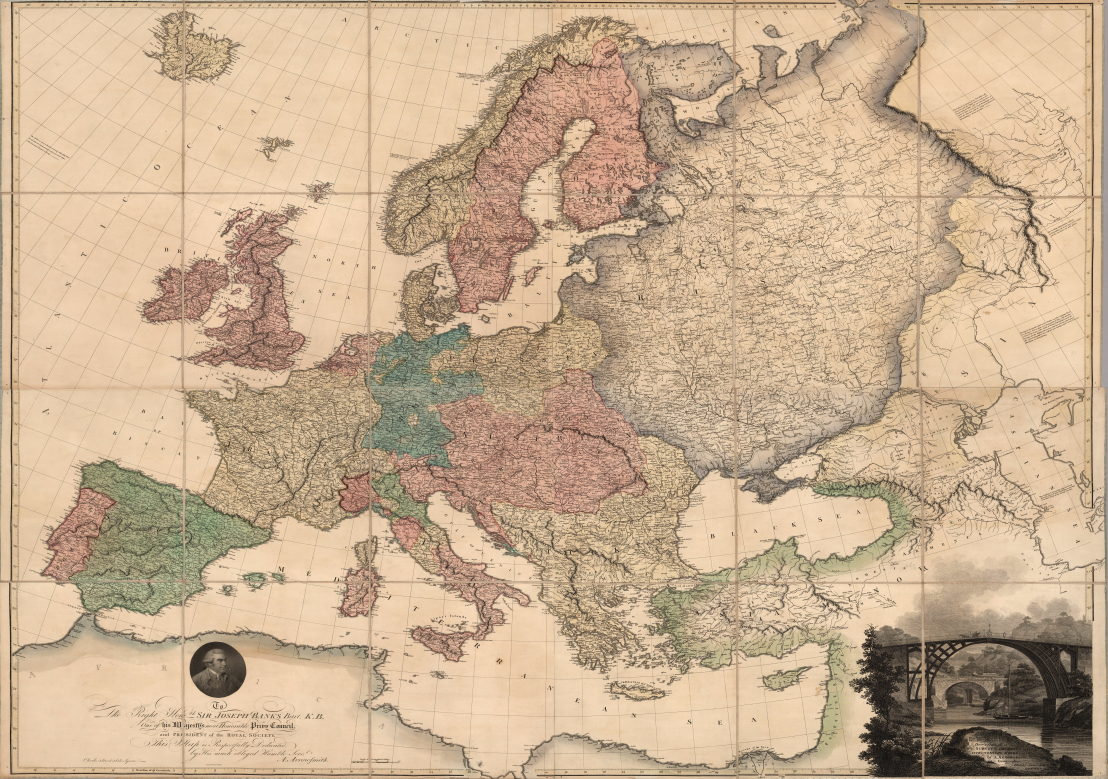
\includegraphics[width=1\linewidth]{mappa_original.png}
  \caption{\textit{Map of Europe - Drawn from all the best surveys and rectified by astronomical observation by} \citet{arrowsmith}}
  \label{fig:map}
\end{figure}
A second source of travel routes is waterways. While maritime and river transport offered the lowest friction for bulk goods, they were not necessarily the fastest for information or passengers before steam. However, they remained essential for heavy industrial inputs.
As industrialization progressed, many canals were constructed and rivers were canalized. To avoid endogeneity, we restrict attention to rivers that were navigable prior to industrialization, excluding canalized or newly constructed waterways.
We construct a GIS dataset of navigable waterways using multiple sources.
Finally, although data on existing railways during this period are available \citep{bogart2014transport}, we exclude them to avoid endogeneity concerns.

The travel cost computation rests on two assumptions:
\begin{enumerate}
  \item Travel cost is symmetric: travelling from location \(i\) to \(j\) costs the same as travelling from \(j\) to \(i\).
  \item Travel cost is constant over the entire period of analysis (1835--1899). This is the strongest assumption, as railway construction and canal improvements substantially reduced travel costs during this period. We impose this restriction to avoid endogeneity concerns (railways were themselves a product of industrialization) but acknowledge it as a limitation to be addressed in future work with time-varying transport networks.
\end{enumerate}
In a rich geography problem, given a matrix of instantaneous speed representing the existing travel network, computing the travel cost between locations \(i\) and \(j\) requires finding the shortest path connecting them. We implement this using a Dijkstra shortest-path algorithm on a 10~km resolution grid covering continental Europe.
We assign base speeds of 4.5~km/h for main roads, 8.0~km/h for sea, 6.0~km/h for navigable waterways, and 2.0~km/h for off-road terrain. These base speeds are then adjusted for terrain slope using the Tobler hiking function, which modulates walking speed as \(v(s) = 6 \exp(-3.5 |s + 0.05|)\)~km/h, where \(s\) is the slope gradient. For each grid cell, we compute a harmonic-mean Tobler multiplier using both uphill and downhill directions to obtain a direction-independent friction surface. Sea-to-land transitions incur an additional overhead of 24~hours to capture port handling costs. The resulting network yields travel times in hours between all NUTS2 centroid pairs.
These speed parameters are informed by the historical transport literature. The off-road speed of 2~km/h reflects the effective pace of goods transport over unimproved terrain: while unloaded walkers reach 5~km/h on flat ground \citep{tobler1993three}, loaded ox-drawn carts averaged roughly 2--3~km/h on rough surfaces \citep{rodrigue2020geography}. The on-road speed of 4.5~km/h captures a blend of freight haulage (3--4~km/h for horse-drawn wagons) and individual travel, consistent with the observation that pre-turnpike stagecoaches averaged 2--3~km/h and improved to about 6~km/h by the 1830s \citep{rodrigue2020geography}. For comparison, \citet{allen2024topography} assigns 5~km/h off-road and reduces travel time by 40\% on Roman roads following \citet{davey1994road}, while \citet{ozak2018distance} uses the Tobler function directly. The sea speed of 8~km/h (\(\approx\)4.3~knots) falls in the lower range of sailing speeds documented in the CLIWOC logbook data for the period 1750--1850 \citep{kelly2019speed}. The waterway speed of 6~km/h represents an average over upstream and downstream navigation on major European rivers. The slope adjustment follows the Tobler hiking function \citep{tobler1993three}, which is widely adopted in spatial cost analysis \citep{ozak2018distance, allen2024topography}.
\begin{figure}[h]
  \centering
  \begin{subfigure}[b]{0.45\textwidth}
    \centering
    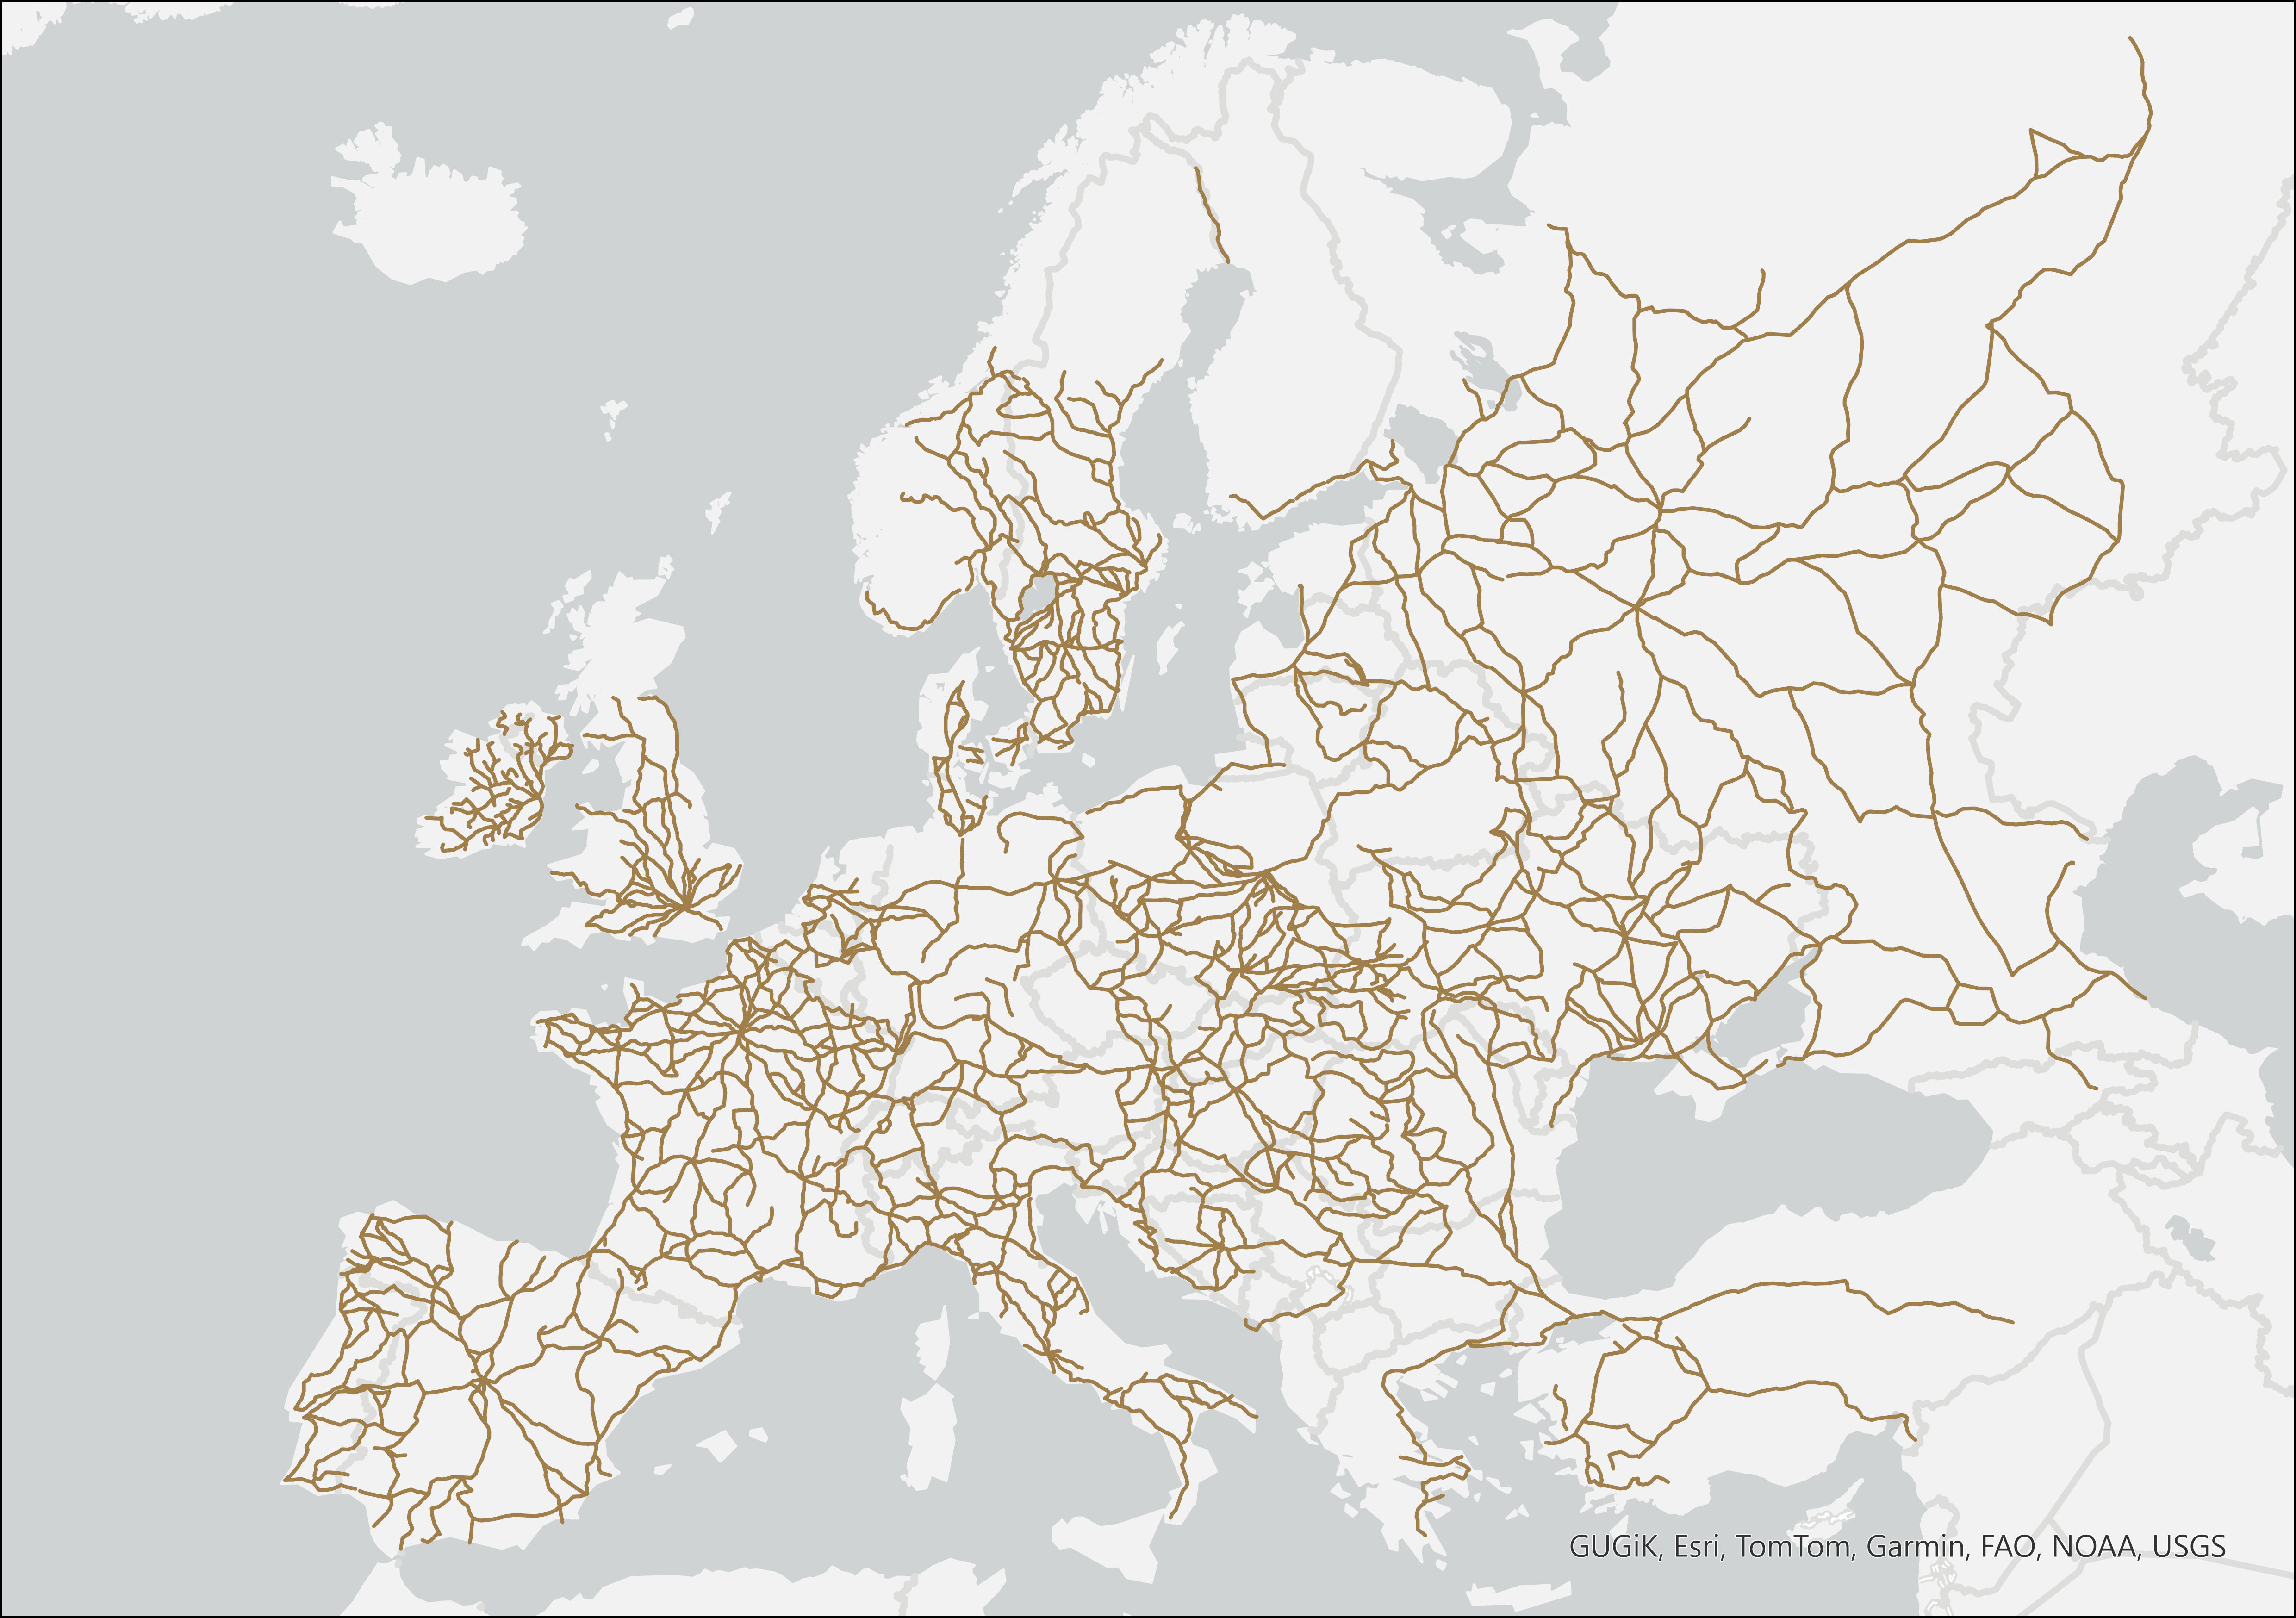
\includegraphics[width=\textwidth]{roads.jpg}
    \caption{Digitized roads}
    \label{fig:roads}
  \end{subfigure}
  \hfill
  \begin{subfigure}[b]{0.45\textwidth}
    \centering
    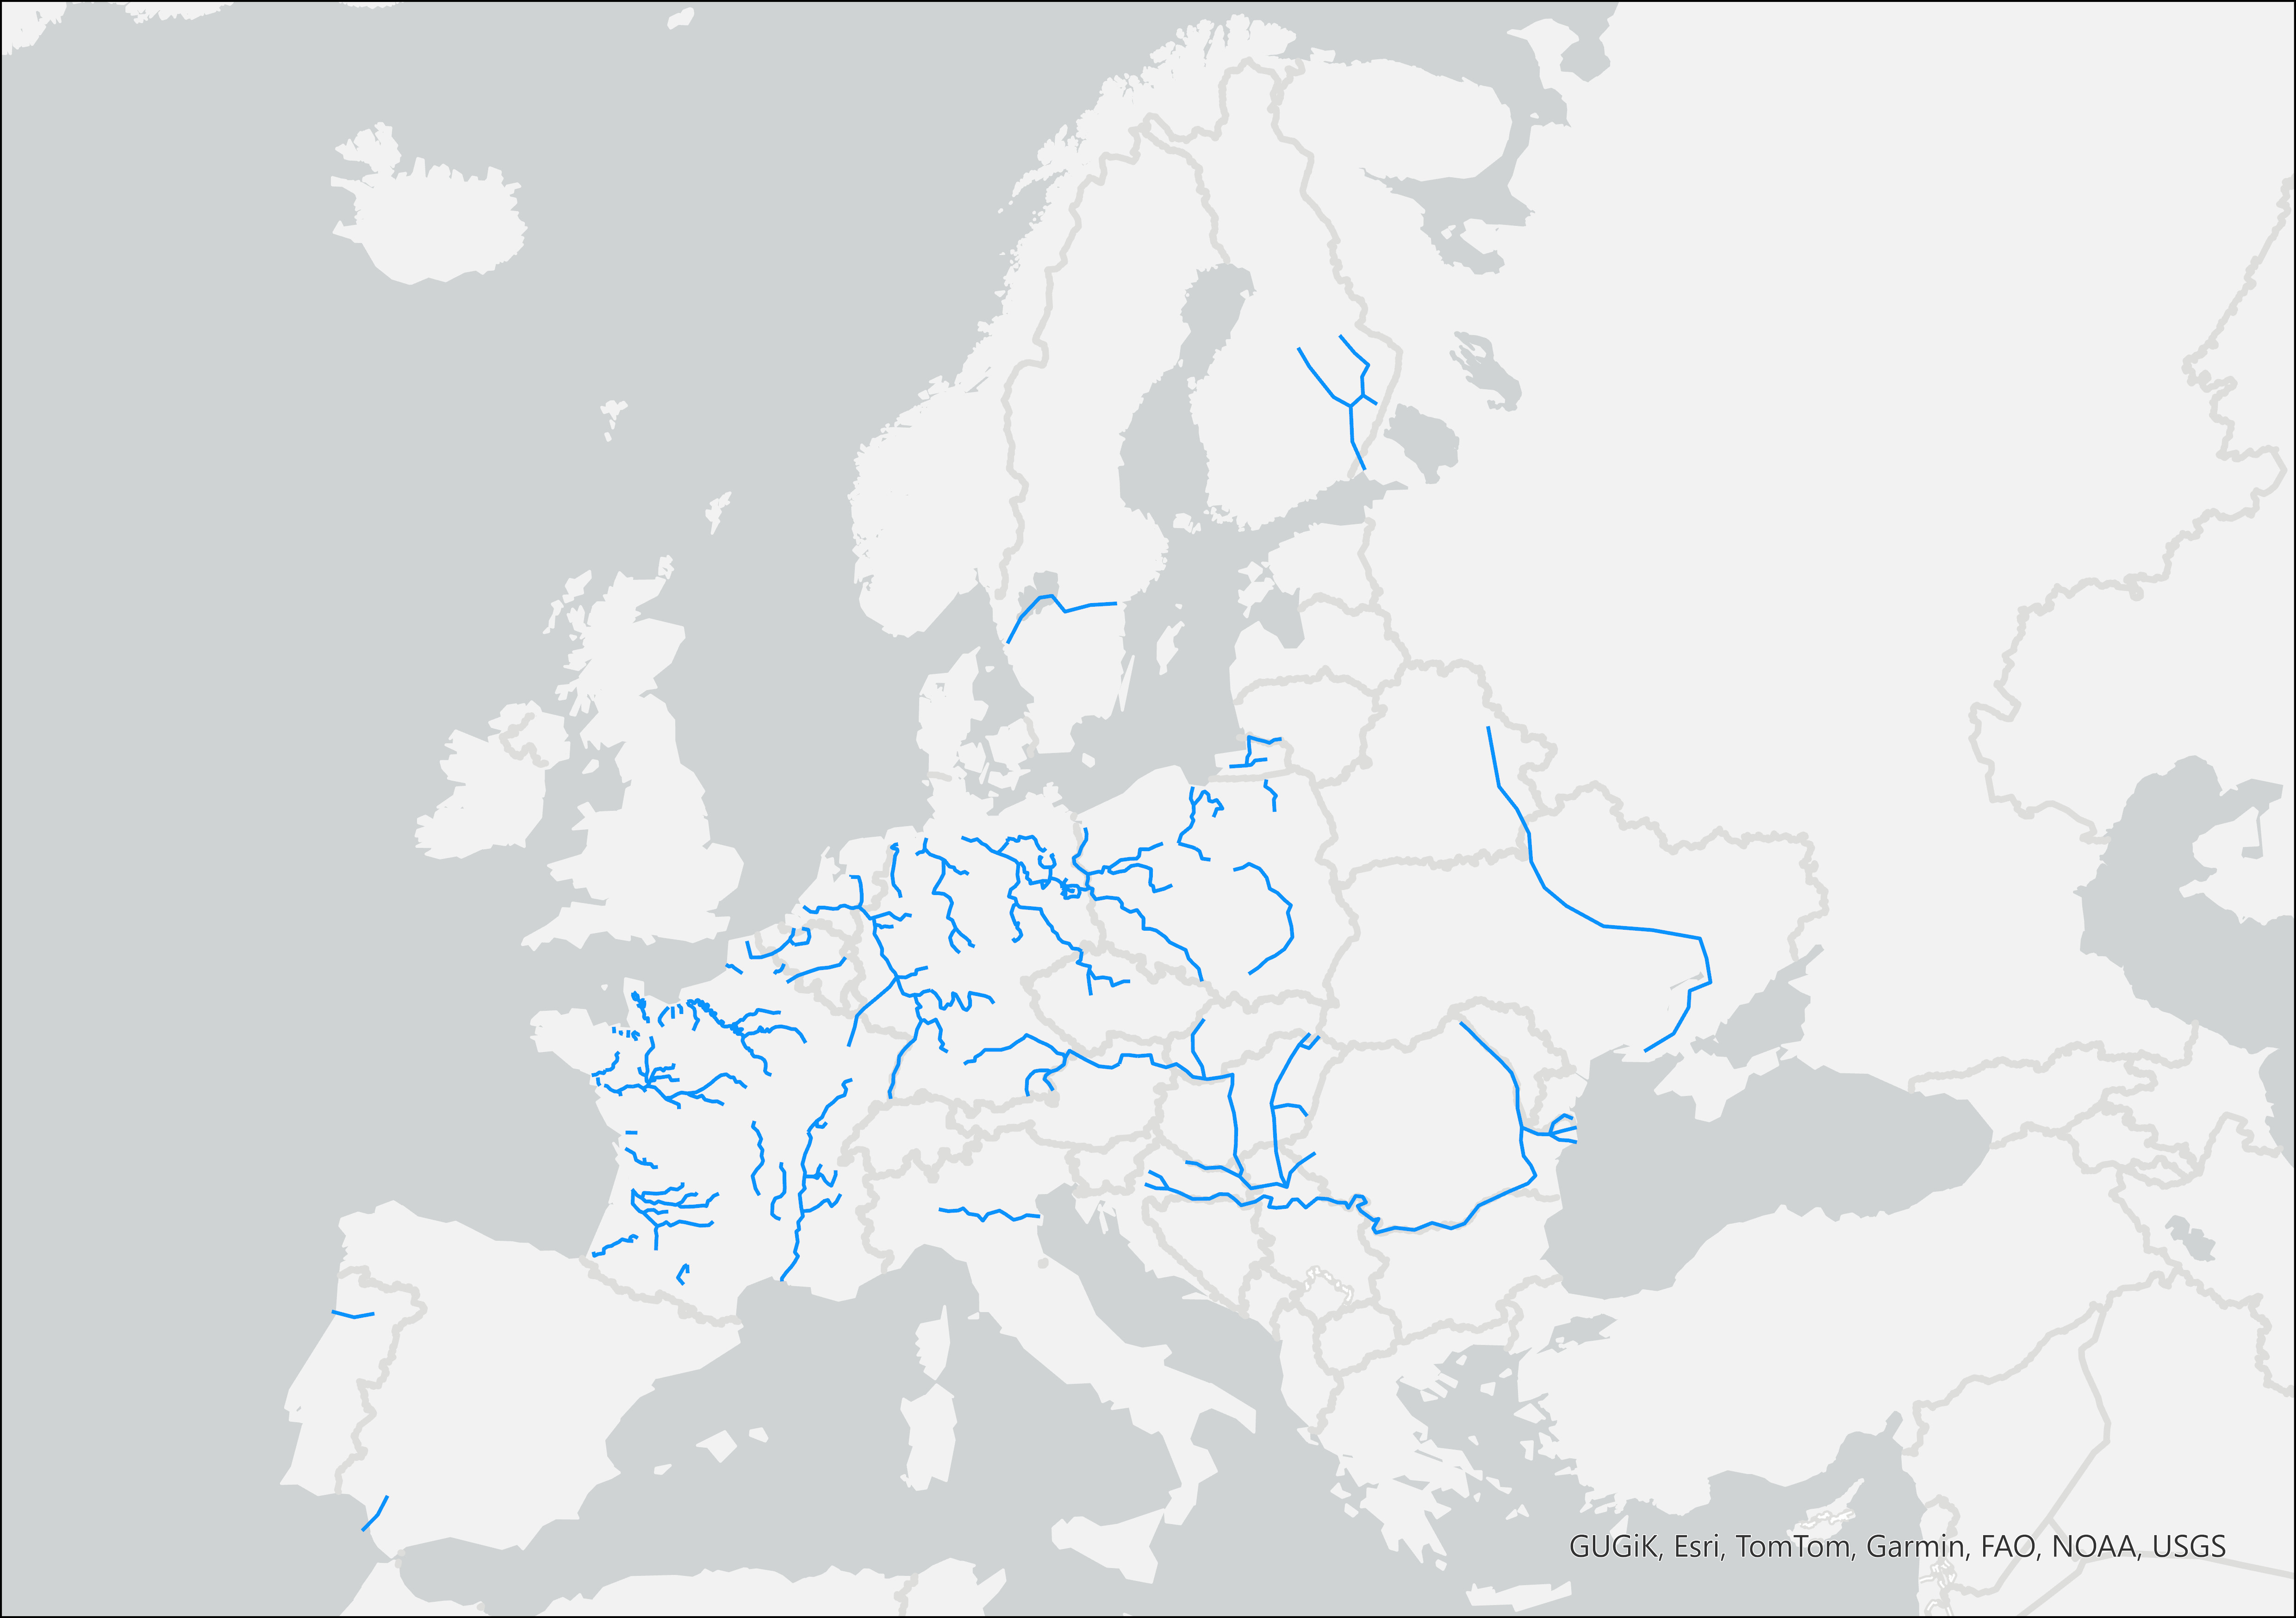
\includegraphics[width=\textwidth]{rivers.jpg}
    \caption{Digitized navigable waterways}
    \label{fig:rivers}
  \end{subfigure}
  \caption{Historical transport network used to construct the friction surface. Roads are digitized from the \citet{arrowsmith} map; waterways include only rivers documented as navigable prior to industrialization.}
  \label{fig:transport_network}
\end{figure}

\subsubsection*{Input prices and Proximity to coal mines}

Transport costs were a major factor influencing coal prices in Europe. For instance, \citet{licio2022coal} reports that in 1870, French coal delivered to Turin had a total price of 35 Italian Lire per ton, with transport costs accounting for a significant 20 Lire, more than half the total price.
\begin{figure}
  \centering
  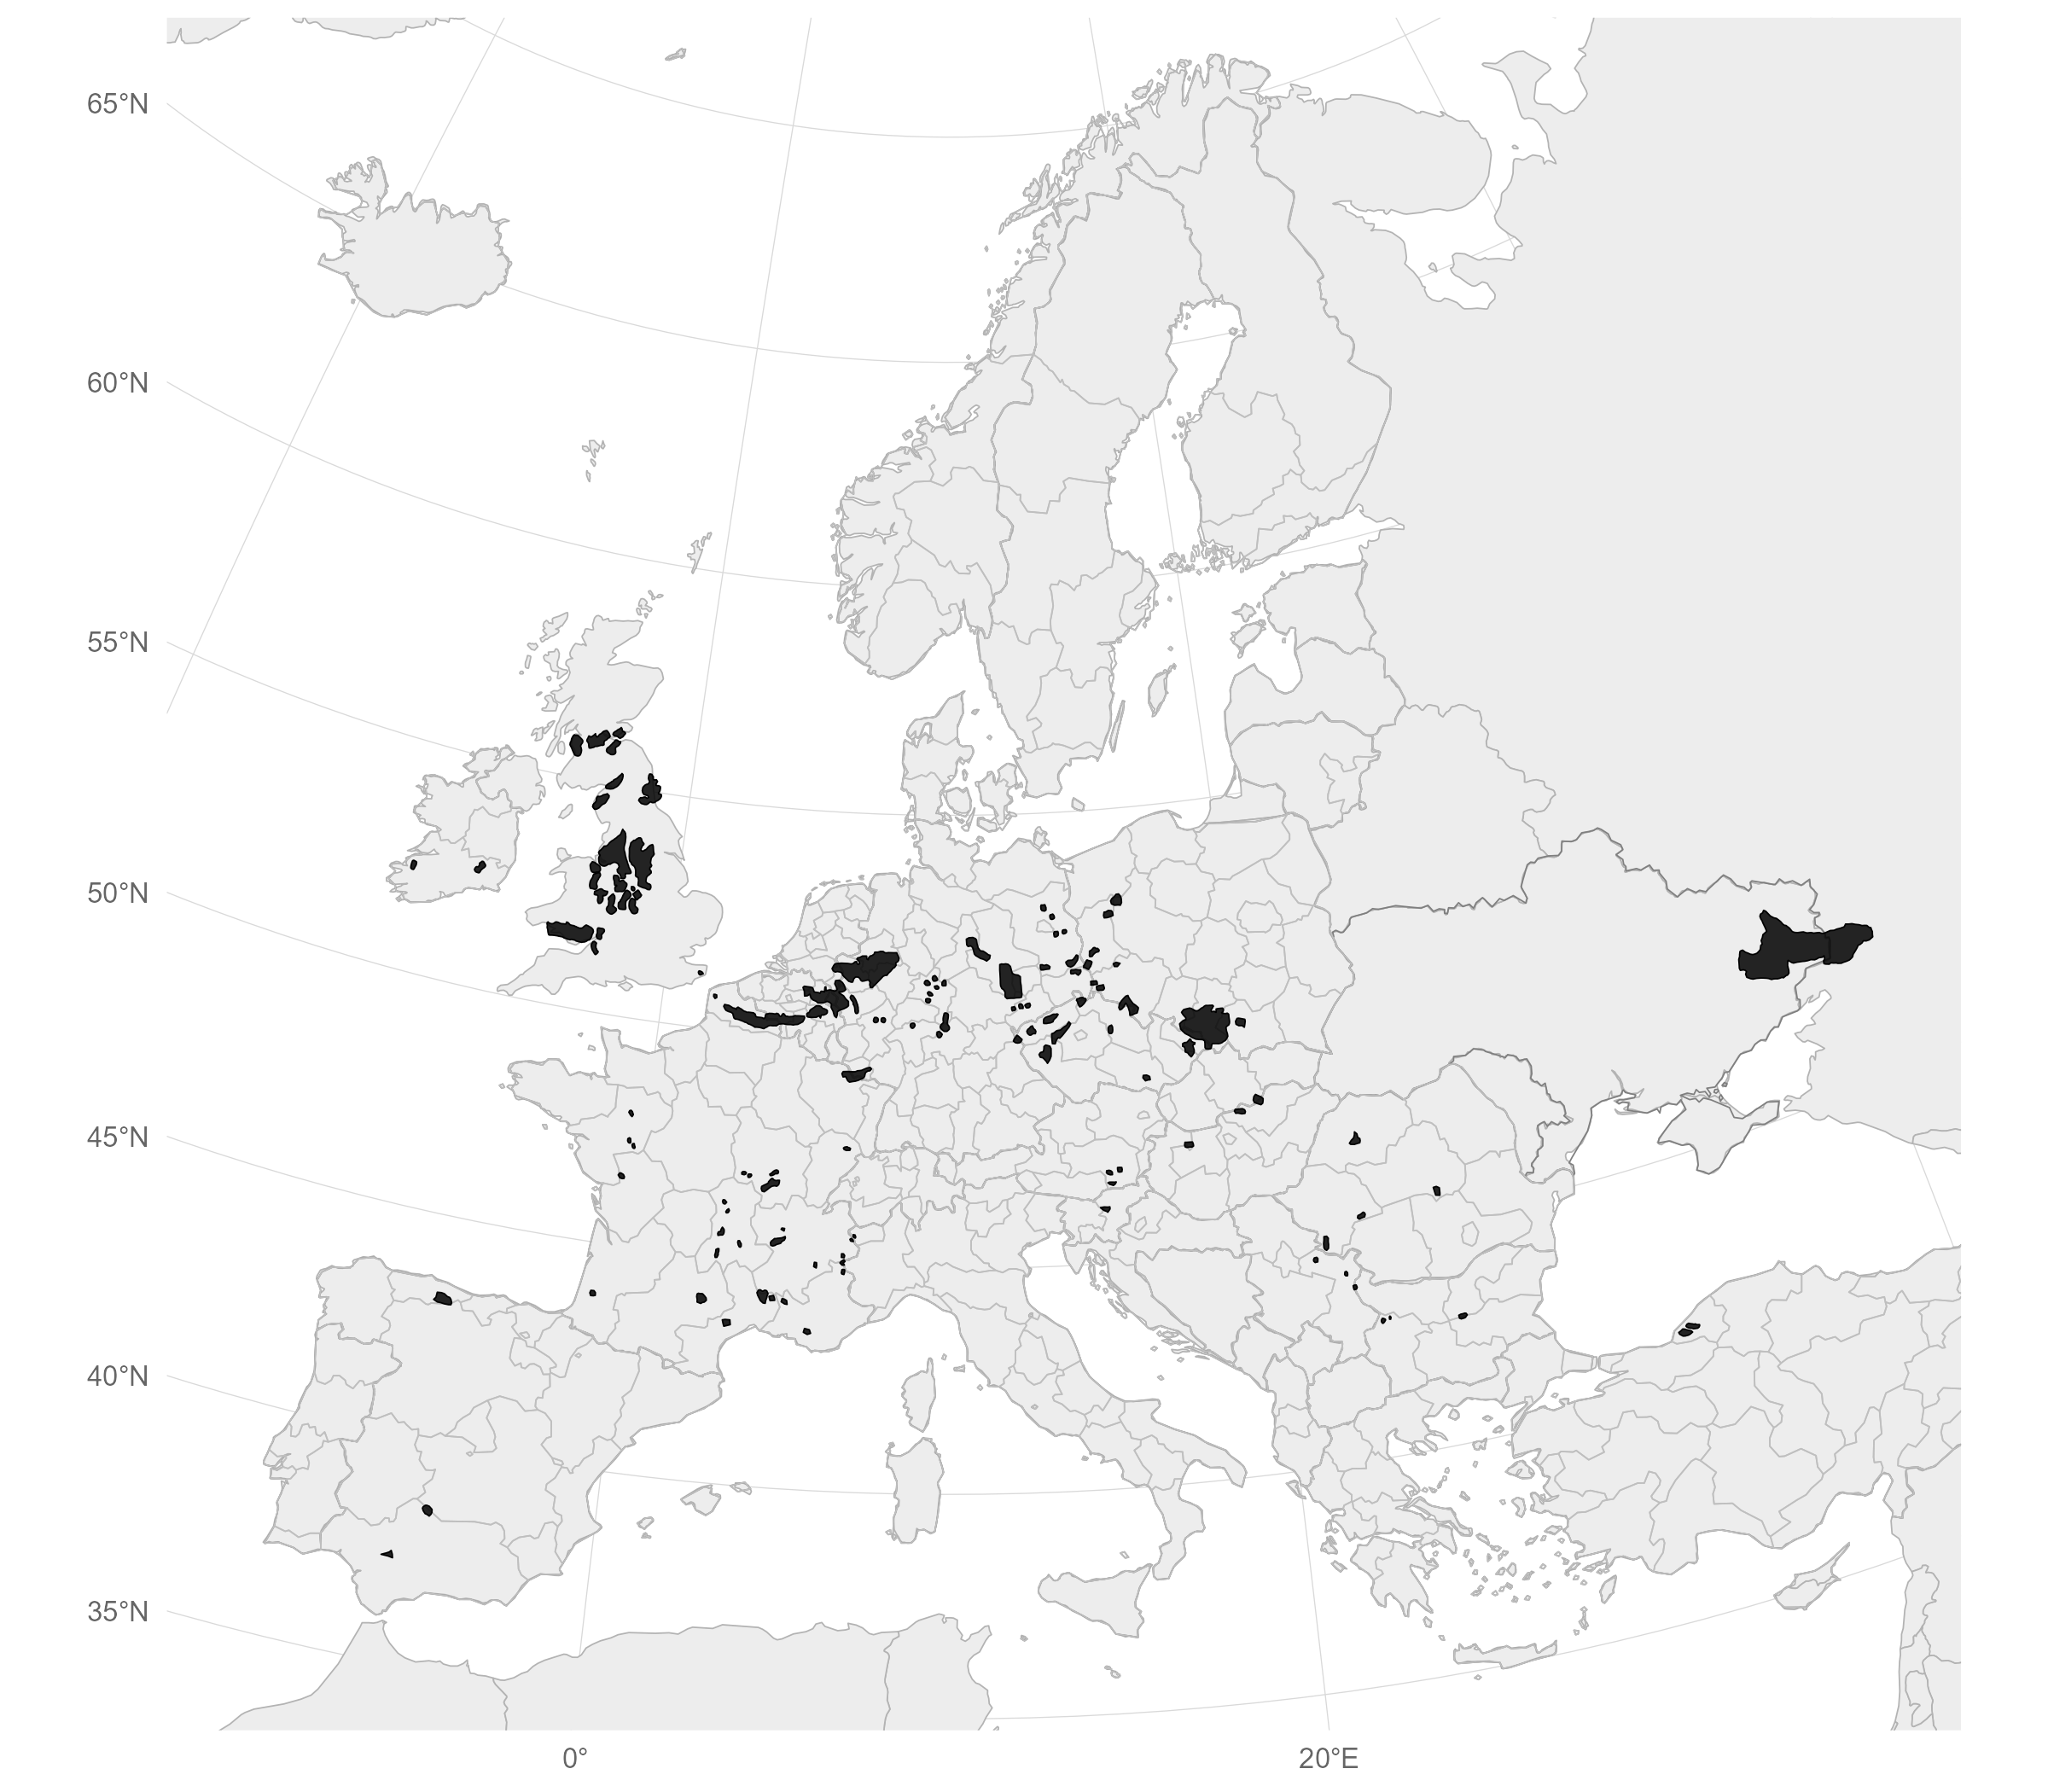
\includegraphics[width=1\linewidth]{coal_mines_map.png}
  \caption{Major coalfields in Europe. Source: author's elaborations from \citet{fernihough2021coal} data. Shapefile from \citet{portotapiquen2015}.}
  \label{fig:coal_mines}
\end{figure}
The impact of transport costs is even more pronounced when considering British coal. Due to the additional maritime shipping expenses, British coal reached a final price of 55 Lire per ton in Turin. Of this total, 43 Lire was attributed to transportation: 28 Lire for sea shipping from Cardiff to Genoa, and an additional 15 Lire for rail transport from Genoa to Turin. These examples show that transport costs, both maritime and overland, determined a large share of coal's final delivered price across European locations.
With some notable exceptions, such as \citet{licio2022coal} for Italy, no high-resolution harmonized coal price dataset exists for all of Europe.
Given the importance of transport costs in determining coal prices, we proxy input costs using proximity to coal mines. For each region \(i\), we compute the minimum travel cost to any coalfield in the sample:
\begin{equation}
  \label{eq:ip}
  IP_i = \min_{m \in \mathcal{M}} TC_{im}
\end{equation}
where \(\mathcal{M}\) is the set of coalfield polygons identified in the data. This specification captures the effective input cost faced by a representative firm: producers source coal from the nearest accessible deposit, so the relevant price is the minimum across all mines. As a robustness check, we replace \(IP_i\) with the mean travel time across all coalfields; Section~\ref{sec:rob_coal} shows that the results are insensitive to this choice.

\subsubsection*{Population estimates}
We estimate population at the NUTS2 level using a dataset of European city populations compiled by \citet{ThePopulationofEuropeanCitiesfrom700to2000}. For our period of analysis, this dataset provides estimates at three benchmark dates: 1800, 1850, and 1900.
To compute regional population aggregates, we sum the city populations within each NUTS2 boundary. While this approach captures only urban population, it provides a consistent measure across regions and time periods.

\subsection{Estimation strategy}

\subsubsection*{From theory to estimating equation}

The knowledge generation function in equation~\eqref{eq:final} cannot be estimated directly because its dependent variable, industrial knowledge (\(ik_{i,t}\)), is unobservable. However, under the assumption that patent production is proportional to knowledge generation, \(P_{i,t} \propto ik_{i,t}\), we can substitute the structural spillover~\eqref{eq:spillover_structural} into equation~\eqref{eq:final} and proxy \(IK\) with \(CP\) to obtain an estimable reduced-form patent equation:

\begin{equation}
  \label{eq:estimable}
  \begin{split}
    P_{i,t} &= \exp\bigl(c_0 + c_1 \ln CP_{i,t-1} + c_2 \ln Pop_{i,t} \\
    &\quad + c_3 \ln S_{i,t}(\alpha, \beta, \phi) + c_4 \ln IP_i + \mu_c + \delta_t \bigr) \cdot \eta_{i,t}
  \end{split}
\end{equation}

\noindent where \(\mu_c\) and \(\delta_t\) are country and time fixed effects, and the reduced-form coefficients are composites of the underlying structural parameters: for instance, \(c_1\) absorbs both the persistence of knowledge (\(\gamma\)) and the patent--knowledge elasticity, while \(c_3\) captures the overall strength of spatial spillovers (\(\varepsilon\)). Country fixed effects absorb time-invariant institutional and geographical characteristics, while time fixed effects capture common shocks such as continent-wide business cycles or technological paradigm shifts.

\subsubsection*{Identification of structural spillover parameters}

While the composite coefficients \(c_0, \ldots, c_4\) do not allow the recovery of all individual structural parameters, the three parameters governing the {\em shape} of the spillover function---\(\alpha\) (destination population elasticity), \(\beta\) (origin population elasticity), and \(\phi\) (knowledge stock elasticity)---enter the model nonlinearly through the spillover index in equation~\eqref{eq:spillover_structural} and can be estimated by concentrated least squares.

\subsubsection*{Two-phase estimation}

We employ a two-phase estimation strategy:

\begin{enumerate}
  \item \textbf{Reduced-form estimation.} We first estimate equation~\eqref{eq:estimable} with a pre-specified linear spillover index (\(\alpha = 0\), \(\beta = 1\), \(\phi = 1\)), yielding \(S_{i,t} = \sum_{j \neq i} Pop_{j,t} \cdot CP_{j,t-1} / T_{ij}\). This provides baseline estimates of the reduced-form coefficients using both OLS and Poisson Pseudo-Maximum Likelihood (PPML) with country and year fixed effects, following the recommendation of \citet{santos2006log} for gravity equations with heteroskedastic errors and zero-valued dependent variables.

  \item \textbf{Structural estimation via concentrated least squares.} We then relax the restrictions on (\(\alpha\), \(\beta\), \(\phi\)) and recover their values by concentrated least squares. The procedure nests two optimization loops: the outer loop searches over \((\alpha, \beta, \phi)\) using the L-BFGS-B algorithm, while for each candidate triplet the inner loop recomputes the spillover \(S_{i,t}(\alpha, \beta, \phi)\) using the full bilateral travel cost matrix and re-estimates the linear coefficients by OLS. The outer loop minimizes the sum of squared residuals. We initialize the search with a grid over a coarse parameter space to mitigate the risk of converging to local minima.
\end{enumerate}

Finally, we complement these intensity models with a Cox proportional hazards model for the {\em timing} of industrialization, using time-invariant regional covariates. Section~\ref{sec:cox_robust} reports targeted sensitivity checks.


\section{Empirical Results}

We adopt a progressive estimation strategy. We begin with reduced-form and structural gravity estimates of patenting intensity, then assess identification and robustness. We then complement these intensity results with a Cox proportional hazards model for the timing of industrialization.

Our dataset consists of a balanced panel of 296 NUTS2 regions observed at decadal frequency from 1840 to 1900, where years denote decade endpoints (e.g., 1900 corresponds to the 1890s). After removing observations with missing population or coal cost data, the estimation sample comprises 2,023 region-decade observations.

\subsection{Reduced-Form Gravity Model}

We begin by estimating equation~\eqref{eq:estimable} under the baseline restrictions \(\alpha = 0\), \(\beta = 1\), \(\phi = 1\), which yield the linear spillover index \(S_{i,t} = \sum_{j \neq i} Pop_{j,t} \cdot CP_{j,t-1} / T_{ij}\). We estimate this specification using both OLS on the log-linearized form and Poisson Pseudo-Maximum Likelihood (PPML) with country and year fixed effects, following the recommendation of \citet{santos2006log} for gravity equations with heteroskedastic errors and zero-valued observations.


\begin{table}[htbp]
   \caption{\label{tab:gravity} Gravity Model Results (OLS \& PPML with Fixed Effects)}
   \centering
   \begin{tabular}{lcc}
      \tabularnewline \midrule \midrule
      Dependent Variables:      & log\_patents  & patents\\  
      Model:                    & (1)           & (2)\\  
                                &  OLS          & Poisson\\  
      \midrule
      \emph{Variables}\\
      Lagged Patent Stock (log) & 0.841$^{***}$ & 0.785$^{***}$\\   
                                & (0.015)       & (0.009)\\   
      Population (log)          & 0.144$^{***}$ & 0.323$^{***}$\\   
                                & (0.013)       & (0.012)\\   
      Spillover index (log)     & 0.074$^{***}$ & 0.020$^{***}$\\   
                                & (0.022)       & (0.005)\\   
      Coal cost (log)           & -0.018        & -0.070$^{***}$\\   
                                & (0.019)       & (0.011)\\   
      \midrule
      \emph{Fixed-effects}\\
      country\_id               & Yes           & Yes\\  
      year                      & Yes           & Yes\\  
      \midrule
      \emph{Fit statistics}\\
      Observations              & 2,023         & 1,974\\  
      Squared Correlation       & 0.85790       & 0.94597\\  
      Pseudo R$^2$              & 0.56545       & 0.93073\\  
      BIC                       & 3,383.6       & 9,748.9\\  
      \midrule \midrule
      \multicolumn{3}{l}{\emph{IID standard-errors in parentheses}}\\
      \multicolumn{3}{l}{\emph{Signif. Codes: ***: 0.01, **: 0.05, *: 0.1}}\\
   \end{tabular}
\end{table}




Table~\ref{tab:gravity} presents the results. The PPML estimates (Model 2) show that all four covariates are highly significant. The elasticity of patents to the lagged knowledge stock is \(0.79\), confirming the cumulative nature of the innovation process. Population enters with an elasticity of \(0.32\), implying diminishing returns to scale in knowledge production. The spillover index is positive and significant (\(+0.02\), \(p < 0.01\)), consistent with spatial knowledge diffusion. Coal access carries a negative coefficient (\(-0.07\), \(p < 0.01\)), consistent with the hypothesis that proximity to energy sources was a determinant of innovation capacity during the Industrial Revolution.

\subsection{Structural Estimation}

The reduced-form specification imposes restrictive assumptions on the structure of knowledge spillovers. In particular, it constrains the elasticities of origin population (\(\alpha\)), destination population (\(\beta\)), and past knowledge (\(\phi\)) to fixed values that may not correspond to the true data-generating process described in equation~\eqref{eq:final}.

To recover these structural parameters, we employ a concentrated least squares approach. The reduced form of our three-equation system (after substituting equation~\eqref{eq:knowledge} into the patent production equation) yields

\begin{equation}
  \label{eq:structural_reduced}
  \begin{split}
    \ln P_{i,t} &= c_0 + c_1 \ln CP_{i,t-1} + c_2 \ln Pop_{i,t} \\
    &\quad + c_3 \ln S_{i,t}(\alpha, \beta, \phi) + c_4 \ln IP_i + \mu_c + \delta_t + \epsilon_{i,t}
  \end{split}
\end{equation}

\noindent where the structural spillover is now

\begin{equation}
  \label{eq:structural_spillover}
  S_{i,t}(\alpha, \beta, \phi) = \sum_{j \neq i} \frac{Pop_{i,t}^{\alpha} \cdot Pop_{j,t}^{\beta} \cdot CP_{j,t-1}^{\phi}}{T_{ij}}
\end{equation}

\noindent and the reduced-form coefficients \(c_0, \ldots, c_4\) are composites of the underlying structural parameters \((\gamma, \eta, \varepsilon, \theta, \lambda, \mu, \omega, \delta)\). The nonlinear parameters \((\alpha, \beta, \phi)\) are, however, separately identified because they enter the model inside the summation operator.

The concentrated least squares procedure works by nesting two optimization loops. In the outer loop, we search over the structural parameters \((\alpha, \beta, \phi)\) using the L-BFGS-B algorithm. For each candidate triplet, we recompute the spillover index \(S_{i,t}(\alpha, \beta, \phi)\) using the full bilateral travel cost matrix and then estimate the linear parameters \((c_0, \ldots, c_4)\) by OLS in an inner loop. The outer loop minimizes the sum of squared OLS residuals. We initialize the optimization using a grid search over a coarse parameter space to avoid local minima. As a robustness check, we also report PPML estimates of the reduced-form patent equation evaluated at the spillover index implied by the estimated structural parameters.

The structural estimation requires computing the bilateral spillover for every region pair, which restricts the sample to the subset of regions present in both the panel dataset and the travel cost matrix. Regions for which the structural spillover evaluates to zero (typically peripheral regions with no patenting neighbors within reach) are also excluded because the log transformation is undefined. These restrictions reduce the estimation sample relative to the reduced-form specification.


\begin{table}
\begin{center}
\begin{tabular}{l c c}
\hline
 & OLS (log patents) & PPML (patents) \\
\hline
Lagged Patent Stock (log)  & $0.84^{***}$ & $0.80^{***}$  \\
                           & $(0.02)$     & $(0.01)$      \\
Population (log)           & $0.17^{***}$ & $0.29^{***}$  \\
                           & $(0.02)$     & $(0.01)$      \\
Structural spillover index (log) & $0.47^{***}$ & $-0.11^{***}$ \\
                           & $(0.08)$     & $(0.04)$      \\
Coal cost (log)            & $0.02$       & $-0.11^{***}$ \\
                           & $(0.02)$     & $(0.01)$      \\
\hline
Num. obs.                  & $1463$       & $1414$        \\
Num. groups: country\_id   & $35$         & $30$          \\
Num. groups: year          & $7$          & $7$           \\
R$^2$ (full model)         & $0.88$       & --            \\
R$^2$ (proj model)         & $0.71$       & --            \\
Adj. R$^2$ (full model)    & $0.88$       & --            \\
Adj. R$^2$ (proj model)    & $0.71$       & --            \\
Deviance                   & --           & $5437.36$     \\
Log Likelihood             & --           & $-3925.20$    \\
Pseudo R$^2$               & --           & $0.93$        \\
\hline
\multicolumn{3}{l}{\scriptsize{$^{***}p<0.01$; $^{**}p<0.05$; $^{*}p<0.1$}}
\end{tabular}
\caption{Structural Gravity Model (Concentrated Least Squares)}
\label{tab:structural}
\end{center}
\end{table}


Table~\ref{tab:structural} reports the estimates of equation~\eqref{eq:structural_reduced} evaluated at the structural spillover index \(S_{i,t}(\hat{\alpha}, \hat{\beta}, \hat{\phi})\). Column~(1) reports OLS estimates of the log-linear specification (with country and year fixed effects), while Column~(2) reports PPML estimates of the corresponding count specification, evaluated at the same spillover index.

The concentrated least squares outer loop yields estimates of the spillover-shape parameters in equation~\eqref{eq:structural_spillover}: \(\hat{\alpha} \approx 0\), \(\hat{\beta} = 1.81\) (SE \(= 0.51\)), and \(\hat{\phi} = 0.25\) (SE \(= 0.11\)), with standard errors computed from the numerical Hessian of the concentrated objective function.\footnote{Block bootstrap standard errors clustered by country (200 replications) yield larger SEs (\(\text{SE}(\hat{\beta}) = 1.16\), \(\text{SE}(\hat{\phi}) = 0.63\)), as expected when accounting for cross-country heterogeneity.} These parameters are not regression coefficients: they enter only through the construction of \(S_{i,t}(\alpha,\beta,\phi)\). An \(F\)-test for \(H_0: \alpha = 0\) yields \(p > 0.99\), confirming that the restriction is not binding. The structural estimation sample drops to 1,463 (OLS) and 1,414 (PPML) observations because regions must be present in the travel cost matrix and must have positive structural spillover values.

Three aspects of these spillover-shape estimates have direct economic interpretation.

First, \(\hat{\alpha} \approx 0\) indicates that the population of the receiving region does not amplify the incoming knowledge spillover. In the context of our model, this means that even small regions could benefit from proximity to innovative hubs, suggesting that geography, rather than market size, determined the ability to absorb external knowledge during this period.

Second, \(\hat{\beta} = 1.81\) (\(t = 3.52\), \(p < 0.01\)) is significantly different from zero, confirming that the population of the source region matters for knowledge generation. The point estimate substantially exceeds unity, suggesting increasing returns to scale in the population of the source region, consistent with strong agglomeration economies in innovation \citep{jaffe1993geographic}.

Third, \(\hat{\phi} = 0.25\) (\(t = 2.19\), \(p < 0.05\)) reveals strongly diminishing returns to accumulated knowledge in the spillover process. This finding is consistent with the ``fishing out'' hypothesis: as the stock of knowledge grows, the marginal contribution of each additional patent to cross-regional spillovers decreases. The first innovations in a region have a higher relative impact on neighboring areas than subsequent ones.

The estimated spillover elasticity \(\hat{c}_3\) (coefficient on the structural spillover index) diverges between OLS (\(+0.47\), \(p < 0.01\)) and PPML (\(-0.11\), \(p < 0.01\)). This sign reversal in the PPML specification may arise because the structural formulation, with its strongly increasing returns to source population (\(\hat{\beta} = 1.81\)), concentrates spillovers among a few large urban centers; the PPML estimator, which places greater weight on observations with large counts, may then attribute the remaining variation to competitive effects rather than diffusion. The OLS estimator, which weights all observations equally in logs, recovers the positive diffusion channel. This pattern is consistent with a model where spillovers operate at the extensive margin (enabling initial industrialization) rather than the intensive margin (driving further patent growth in already-innovative regions).

\subsection{Identification and Endogeneity}
\label{sec:endogeneity}

A potential concern with gravity models of knowledge diffusion is the endogeneity of the main explanatory variables. In particular, we address three specific threats to identification: (1) reverse causality between population growth and innovation, (2) dynamic panel bias (Nickell bias) arising from the lagged dependent variable, and (3) unobserved path dependence where initial advantages drive long-run outcomes.

\begin{table}[!htbp]
\centering
\resizebox{\textwidth}{!}{%
\begin{tabular}{lcccccc}
\hline
\hline
 & Baseline & No CP lag & Pop 1800 & No CP+Pop1800 & InitCP (1850) & InitCP+Pop1800 \\
 & (1) & (2) & (3) & (4) & (5) & (6) \\
\hline
Lagged Patent Stock (log) & $0.785^{***}$ &  & $0.895^{***}$ &  &  &  \\
 & (0.017) &  & (0.015) &  &  &  \\
Population (log) & $0.323^{***}$ & $1.275^{***}$ &  &  & $0.804^{***}$ &  \\
 & (0.023) & (0.030) &  &  & (0.021) &  \\
Spillover Index (log) & $0.020^{**}$ & $-0.037^{**}$ & $0.034^{***}$ & $-0.011$ & $-0.031^{***}$ & $-0.006$ \\
 & (0.009) & (0.018) & (0.009) & (0.023) & (0.011) & (0.012) \\
Coal Cost (log) & $-0.070^{***}$ & $0.138^{***}$ & $-0.119^{***}$ & $-0.008$ & $-0.141^{***}$ & $-0.283^{***}$ \\
 & (0.022) & (0.038) & (0.023) & (0.046) & (0.026) & (0.028) \\
Population 1800 (log) &  &  & $0.192^{***}$ & $1.330^{***}$ &  & $0.755^{***}$ \\
 &  &  & (0.025) & (0.049) &  & (0.027) \\
Initial CP (log) &  &  &  &  & $0.740^{***}$ & $0.963^{***}$ \\
 &  &  &  &  & (0.025) & (0.027) \\
\hline
Observations & 2023 & 2023 & 2023 & 2023 & 2023 & 2023 \\
\hline
\hline
\end{tabular}
}
\caption{Endogeneity Robustness Checks}
\label{tab:robustness}
\end{table}


Table~\ref{tab:robustness} reports PPML estimates of the baseline gravity patent equation under alternative specifications (all with country and year fixed effects). Column~(1) reproduces the baseline model. Column~(2) drops the lagged patent stock. Column~(3) replaces contemporaneous population with population in 1800. Column~(4) combines Columns~(2) and~(3). Column~(5) controls for initial patent stock (cumulated patents up to 1850). Column~(6) combines initial patent stock and population in 1800.

First, the positive relationship between population and patenting in our baseline model (Column~1: \(\beta_{pop} = 0.323\)) could reflect reverse causality: successful industrial clusters attract migration, inflating the population of innovative regions. To gauge this concern, we replace the contemporaneous population with its predetermined 1800 value (Columns~3 and~4). The distribution of European population in 1800 predates the major wave of industrialization and railway construction; it is therefore plausibly free from contamination by late-19th-century innovation shocks and remains highly predictive of subsequent settlement patterns. We note that this approach does not constitute a formal instrumental variable strategy (it replaces a potentially endogenous regressor with a predetermined control) and therefore does not fully resolve reverse causality. Nevertheless, it provides a useful diagnostic.
Table~\ref{tab:robustness} (Column~3) shows that when using population in 1800, the spillover coefficient increases to \(+0.034\) (\(p < 0.01\)) and remains highly significant (on the same 2,023 observations). This suggests that our baseline findings are not driven by endogenous migration; if anything, the baseline estimate appears conservative.

Second, we address the concern of Nickell bias. In a fixed-effects model with a lagged dependent variable (knowledge stock), the estimates can be biased in finite samples. Column 2 (R1) drops the lagged stock entirely; this removes the Nickell bias but also omits the region's own absorptive capacity.
The results show that without controlling for the region's own history, the spillover coefficient turns negative (Column~2: \(-0.037\), \(p < 0.05\)). This indicates that the positive spillover effect is conditional on a region's accumulated capabilities: among regions with similar populations, those surrounded by innovation but lacking their own knowledge stock tend to patent \textit{less}, possibly due to competition or agglomeration shadows. The positive diffusion channel (\(+0.02\)) is only revealed when we account for the region's own dynamic path; the baseline result is therefore not a mechanical artifact of the lagged dependent variable but a conditional economic relationship.

Third, we explore the role of path dependence. A critique of spatial diffusion models is that they may simply capture the persistence of initial advantages: regions that were innovative or well-connected early on continued to be so by the end of the sample. To test this, we explicitly control for the initial patent stock accumulated up to 1850 (Columns~5 and~6).
When controlling for initial conditions, the spillover coefficient turns negative (Column~5: \(-0.031\), \(p < 0.01\)) and becomes small and statistically insignificant once we also use predetermined population (Column~6: \(-0.006\)). This reveals that part of the aggregate ``diffusion'' observed in the baseline model reflects the amplification of early locational advantages. Once we condition on the ``starting line,'' the residual spatial interaction appears weaker and potentially competitive or displacing.

\subsection{Robustness: Institutional Controls}

A potential concern with the baseline gravity specification is the omission of institutional quality. If countries with stronger democratic institutions also happen to be located near the British epicenter, the spillover coefficient could be capturing institutional rather than geographic effects.

To address this concern, we augment the gravity model with a measure of institutional quality from the Polity5 dataset \citep{marshall2019polity}. Specifically, we use the \emph{Institutionalized Democracy} score (\texttt{democ}), which ranges from 0 (no democratic features) to 10 (full democracy) and captures the competitiveness of political participation, the openness and competitiveness of executive recruitment, and the constraints on executive authority. This composite score is available at the country level for all major European states---including pre-unification polities such as Prussia, Sardinia, and the Two Sicilies---throughout our period of analysis. We log-transform the variable as \(\log(\texttt{democ} + 1)\) and merge it into our panel at the decadal level.


\begin{table}[htbp]
   \caption{\label{tab:institutions} Institutional Controls}
   \centering
   \begin{tabular}{lccc}
      \tabularnewline \midrule \midrule
      Dependent Variable: & \multicolumn{3}{c}{patents}\\
      Model:                    & (1)             & (2)             & (3)\\  
      \midrule
      \emph{Variables}\\
      Lagged Patent Stock (log) & 0.7870$^{***}$  & 0.7911$^{***}$  & 0.8966$^{***}$\\   
                                & (0.0086)        & (0.0087)        & (0.0054)\\   
      Population (log)          & 0.3215$^{***}$  & 0.3169$^{***}$  & 0.1483$^{***}$\\   
                                & (0.0119)        & (0.0120)        & (0.0068)\\   
      Spillover Index (log)     & 0.0203$^{***}$  & 0.0214$^{***}$  & 0.0850$^{***}$\\   
                                & (0.0046)        & (0.0046)        & (0.0041)\\   
      Coal Cost (log)           & -0.0705$^{***}$ & -0.0712$^{***}$ & -0.2222$^{***}$\\   
                                & (0.0111)        & (0.0111)        & (0.0086)\\   
      Democracy Score (log)     &                 & -0.1709$^{***}$ & -0.0774$^{***}$\\   
                                &                 & (0.0343)        & (0.0138)\\   
      \midrule
      \emph{Fixed-effects}\\
      country\_id               & Yes             & Yes             & \\  
      year                      & Yes             & Yes             & Yes\\  
      \midrule
      \emph{Fit statistics}\\
      Observations              & 1,837           & 1,837           & 1,844\\  
      Squared Correlation       & 0.94605         & 0.94492         & 0.92300\\  
      Pseudo R$^2$              & 0.93028         & 0.93046         & 0.90874\\  
      BIC                       & 9,518.2         & 9,500.7         & 12,221.8\\  
      \midrule \midrule
      \multicolumn{4}{l}{\emph{IID standard-errors in parentheses}}\\
      \multicolumn{4}{l}{\emph{Signif. Codes: ***: 0.01, **: 0.05, *: 0.1}}\\
   \end{tabular}
\end{table}




Table~\ref{tab:institutions} presents three specifications. The first column reproduces the baseline PPML estimates on the sample with non-missing institutional data (\(n = 1{,}837\)). The second column adds the democracy score as an additional covariate while retaining country and year fixed effects; the third column removes country fixed effects entirely, so that institutions absorb the cross-country variation previously captured by the fixed effects.

The democracy score enters with a negative and significant coefficient in both specifications: \(-0.17\) (\(p < 0.01\)) with country fixed effects and \(-0.08\) (\(p < 0.01\)) without. In the specification with country fixed effects (Column 2), identification comes entirely from within-country variation over time: the coefficient captures whether decades of expanding democratic participation \textit{within} a given country coincided with higher patenting, conditional on knowledge stocks, population, and spillover exposure. The negative estimate indicates that they did not. The major waves of constitutional and franchise reform in 19th-century Europe---the revolutions of 1848, the Reform Acts in Britain, and the unification-era constitutional changes in Germany and Italy---were concentrated in specific decades that do not coincide with the steepest increases in patent intensity; if anything, periods of political upheaval may have temporarily disrupted the stable institutional environment that patenting requires. In the specification without country fixed effects (Column 3), the coefficient shrinks to \(-0.08\), as the negative within-country gradient is partially offset by cross-country variation: some of the least democratic states (Russia, the Ottoman Empire) also had the lowest knowledge stocks and spillover exposure, attenuating the negative relationship in levels.

The coefficients on our variables of interest---lagged patent stock, population, spillover index, and coal cost---remain virtually unchanged across all three specifications. The spillover coefficient moves from \(+0.020\) to \(+0.021\) when institutional controls are added. This stability confirms that the spatial diffusion mechanism captured by our gravity model is robust to the inclusion of institutional quality and is not an artifact of omitted institutional heterogeneity.

\subsection{Robustness: Spatial Autocorrelation}

A natural concern with any spatial diffusion model is that the spillover coefficient may reflect residual spatial autocorrelation rather than a genuine causal mechanism. In our setting, the spillover index is by construction a spatially weighted variable; we therefore test whether its significance is inflated by correlated residuals across neighboring regions.

We address this concern through two complementary diagnostics. First, we compute Moran's \(I\) statistics on the PPML residuals for each decade, using \(k\)-nearest-neighbor spatial weights (\(k = 5\)). The results reveal modest but significant residual spatial autocorrelation in the decades of most rapid industrial diffusion (1850, 1870, 1880), while the early and late periods show no significant spatial pattern. This pattern is consistent with a correctly specified diffusion model: the spatial structure is largely absorbed by the spillover variable, but some residual clustering persists during the peak of the diffusion wave.

Second, we re-estimate standard errors using Conley's \citeyearpar{conley1999gmm} spatial HAC estimator (500~km cutoff) and compare them with standard errors clustered by country. Table~\ref{tab:conley} presents the results: coefficients are stable, while the spillover term remains positive but becomes statistically insignificant once spatial or country-level dependence is accounted for.

This attenuation is expected and we believe it does not invalidate the spillover mechanism. As noted by \citet{head2014gravity}, in gravity models of trade and knowledge flows, the spatial structure is the phenomenon under study, not a nuisance parameter. Conley standard errors penalize precisely the spatial correlation that the diffusion variable is designed to capture; they therefore provide a conservative lower bound on significance. The fact that the coefficient remains positive and economically meaningful (\(+0.021\)) across all specifications, despite losing statistical significance under the most conservative corrections, suggests that geographic proximity to innovative centers contributed to patenting activity, though the evidence is not robust to spatial clustering adjustments.


\begin{table}
\begin{center}
\begin{footnotesize}
\begin{tabular}{l@{} c@{} c@{} c@{}}
\toprule
 & IID SE & \shortstack{Conley SE\\(500km)} & \shortstack{Clustered\\SE} \\
\midrule
Lagged Patent Stock (log) & $0.7911^{***}$  & $0.7911^{***}$ & $0.7911^{***}$ \\
                          & $(0.0087)$      & $(0.0562)$     & $(0.0565)$     \\
Population (log)          & $0.3169^{***}$  & $0.3169^{***}$ & $0.3169^{***}$ \\
                          & $(0.0119)$      & $(0.0843)$     & $(0.0813)$     \\
Spillover Index (log)     & $0.0214^{***}$  & $0.0214$       & $0.0214$       \\
                          & $(0.0046)$      & $(0.0161)$     & $(0.0133)$     \\
Coal Cost (log)           & $-0.0712^{***}$ & $-0.0712^{*}$  & $-0.0712^{*}$  \\
                          & $(0.0111)$      & $(0.0398)$     & $(0.0370)$     \\
Democracy Score (log)     & $-0.1709^{***}$ & $-0.1709$      & $-0.1709$      \\
                          & $(0.0343)$      & $(0.2862)$     & $(0.2947)$     \\
\midrule
Num. obs.                 & $1837$          & $1837$         & $1837$         \\
Num. groups: country\_id  & $25$            & $25$           & $25$           \\
Num. groups: year         & $7$             & $7$            & $7$            \\
Deviance                  & $6317.7827$     & $6317.7827$    & $6317.7827$    \\
Log Likelihood            & $-4615.0683$    & $-4615.0683$   & $-4615.0683$   \\
Pseudo R$^2$              & $0.9299$        & $0.9299$       & $0.9299$       \\
\bottomrule
\multicolumn{4}{l}{\tiny{$^{***}p<0.01$; $^{**}p<0.05$; $^{*}p<0.1$}}
\end{tabular}
\end{footnotesize}
\caption{Gravity Model: Standard Errors Comparison}
\label{tab:conley}
\end{center}
\end{table}


\subsection{Robustness: Coal Cost Specification}
\label{sec:rob_coal}

Our baseline proxies input costs with the minimum travel time from each NUTS2 centroid to the nearest coalfield (equation~\eqref{eq:ip}). An alternative is to use the mean travel time across all coalfields, which weights the cost index by the full spatial distribution of coal deposits rather than by the single nearest source. While the minimum is the more natural economic concept (firms optimise over their sourcing options), the mean provides a useful check on whether results are sensitive to the tails of the coal geography (e.g., a few outlying mines that happen to be very close to some regions).

Table~\ref{tab:rob_coal} compares two coal-access measures: the baseline minimum travel time to the nearest coalfield (Columns~1--2) versus the mean travel time across all coalfields (Columns~3--4). The coefficients on the lagged patent stock, population, and the spillover index are stable across all four columns. For coal access, the PPML estimates are negative and statistically significant under both measures: \(-0.070\) (\(p < 0.01\)) with minimum travel time and \(-0.348\) (\(p < 0.01\)) with mean travel time. The OLS coefficient under minimum travel time is small and statistically insignificant (\(-0.018\)), while the OLS coefficient under mean travel time is negative and marginally significant (\(-0.149\), \(p < 0.10\)). Since PPML is our preferred estimator for count data with many zeros, as recommended by \citet{santos2006log}, the consistent sign and significance in Columns~2 and~4 support the robustness of the input-cost channel. The larger elasticity under the mean measure reflects its broader dispersion: minimum travel time is mechanically compressed toward zero for regions located near a coalfield, while mean travel time retains more cross-sectional variation. Overall, the mean-based specification is a stronger version of the same qualitative result: regions with higher coal access costs tended to patent less, regardless of how coal access is measured.


\begin{table}[htbp]
   \caption{\label{tab:rob_coal} Robustness: Coal Cost Specification. Columns 1--2 use minimum travel time to the nearest coalfield (baseline); Columns 3--4 replace it with mean travel time across all coalfields.}
   \centering
   \begin{tabular}{lcccc}
      \tabularnewline \midrule \midrule
      Dependent Variables:           & log\_patents  & patents        & log\_patents  & patents\\  
      Model:                         & (1)           & (2)            & (3)           & (4)\\  
                                     &  OLS          & Poisson        & OLS           & Poisson\\  
      \midrule
      \emph{Variables}\\
      Lagged patent stock (log)      & 0.841$^{***}$ & 0.785$^{***}$  & 0.840$^{***}$ & 0.765$^{***}$\\   
                                     & (0.015)       & (0.009)        & (0.015)       & (0.009)\\   
      Population (log)               & 0.144$^{***}$ & 0.323$^{***}$  & 0.141$^{***}$ & 0.340$^{***}$\\   
                                     & (0.013)       & (0.012)        & (0.013)       & (0.011)\\   
      Spillover index (log)          & 0.074$^{***}$ & 0.020$^{***}$  & 0.072$^{***}$ & 0.026$^{***}$\\   
                                     & (0.022)       & (0.005)        & (0.021)       & (0.004)\\   
      Coal cost: min distance (log)  & -0.018        & -0.070$^{***}$ &               &   \\   
                                     & (0.019)       & (0.011)        &               &   \\   
      Coal cost: mean distance (log) &               &                & -0.149$^{*}$  & -0.348$^{***}$\\   
                                     &               &                & (0.090)       & (0.067)\\   
      \midrule
      \emph{Fixed-effects}\\
      country\_id                    & Yes           & Yes            & Yes           & Yes\\  
      year                           & Yes           & Yes            & Yes           & Yes\\  
      \midrule
      \emph{Fit statistics}\\
      Observations                   & 2,023         & 1,974          & 2,023         & 1,974\\  
      Squared Correlation            & 0.85790       & 0.94597        & 0.85803       & 0.94473\\  
      Pseudo R$^2$                   & 0.56545       & 0.93073        & 0.56572       & 0.93065\\  
      BIC                            & 3,383.6       & 9,748.9        & 3,381.8       & 9,761.0\\  
      \midrule \midrule
      \multicolumn{5}{l}{\emph{IID standard-errors in parentheses}}\\
      \multicolumn{5}{l}{\emph{Signif. Codes: ***: 0.01, **: 0.05, *: 0.1}}\\
   \end{tabular}
\end{table}




\subsection{Cox Hazard Model: Timing of Industrialization}
\label{sec:cox}

While the gravity models capture the determinants of innovation {\em intensity}, they do not directly address the question of {\em when} a region crosses the patenting intensity threshold that we interpret as industrial take-off. To study the timing of industrial take-off, we define the industrialization event using the KDE-derived patent density threshold described in Section~\ref{sec:kde}: a region is considered to have industrialized in the first decade in which its patent density exceeds the threshold value, and regions that never cross the threshold by 1899 are right-censored at 1900. We then estimate a Cox proportional hazards model of the form

\begin{equation}
  h(t \mid \mathbf{x}_i) = h_0(t) \exp(\boldsymbol{\gamma}' \mathbf{x}_i)
\end{equation}

\noindent where \(h(t \mid \mathbf{x}_i)\) is the hazard rate of industrialization for region \(i\), \(h_0(t)\) is the baseline hazard, and \(\mathbf{x}_i\) is a vector of time-invariant regional characteristics including distance from London, a circular encoding of bearing from London (sine and cosine), mean population, and coal access cost. We measure distance from London in two ways: straight-line (Euclidean) distance and friction-surface travel time computed from the historical transport network constructed above. The latter measure accounts for the fact that regions at the same Euclidean distance from London could face very different effective communication costs depending on their access to roads and navigable waterways; this distinction is particularly relevant for understanding the south-eastward trajectory of diffusion documented above.


\begin{table}
\begin{center}
\begin{tabular}{l c}
\hline
 & Estimate \\
\hline
Distance from London (log) & $-2.786^{***}$ \\
 & $(0.187)$ \\
Bearing from London (sin) & $0.336^{*}$ \\
 & $(0.198)$ \\
Bearing from London (cos) & $-0.538^{***}$ \\
 & $(0.183)$ \\
Mean population (log) & $0.110^{*}$ \\
 & $(0.064)$ \\
Coal cost (log) & $-0.197^{**}$ \\
 & $(0.088)$ \\
\hline
AIC              & $1858.99$ \\
R$^2$            & $0.72$ \\
Num. events      & $228$ \\
Num. obs.        & $249$ \\
PH test (global) & $0.002$ \\
\hline
\multicolumn{2}{l}{\scriptsize{$^{***}p<0.01$; $^{**}p<0.05$; $^{*}p<0.1$}}
\end{tabular}
\caption{Cox Hazard Model Results}
\label{tab:cox}
\end{center}
\end{table}


Table~\ref{tab:cox} presents the results using Euclidean distance as a starting point. Distance from London is the dominant predictor of delayed industrialization: the coefficient of \(-2.79\) (\(p < 0.01\)) implies that doubling the distance from London reduces the hazard of industrialization by roughly 86\%. To respect the circular nature of direction, bearing from London enters through its sine and cosine; these directional terms are jointly significant (\(p < 0.01\)), consistent with a south-eastward component of diffusion. Mean population is marginally significant (\(p < 0.10\)), while coal access remains negatively associated with industrialization timing (\(-0.20\), \(p < 0.05\)).

Crucially, when we replace Euclidean distance with friction-surface travel time, the proximity effect remains the dominant predictor. This is a stronger result: travel time captures the actual communication costs faced by 19th-century agents---shaped by existing roads, navigable rivers, and terrain---rather than mere geographic position. The fact that the south-eastward diffusion pattern holds under this measure suggests that the historical transport network, which connected the British core to northern France, Belgium, and the Rhineland more efficiently than to equidistant regions in other directions, actively channeled the spread of inventive knowledge.

The Cox model relies on the proportional hazards (PH) assumption, i.e., covariate effects are time-invariant and hazard ratios are constant over time. The global proportional hazards test yields \(p < 0.01\), suggesting that the PH assumption is violated overall. Covariate-specific tests suggest that non-proportionality is driven primarily by the directional component and coal access, while the distance effect itself satisfies the PH test. Section~\ref{sec:cox_robust} reports a targeted sensitivity check that addresses this issue.

\subsection{Robustness: Cox Specification}
\label{sec:cox_robust}

The baseline Cox model (Table~\ref{tab:cox}) yields a global PH-test \(p\)-value of \(0.002\), indicating some departure from proportional hazards. To verify that our key result is not an artifact of this violation, we re-estimate the Cox model allowing time-varying coefficients for the covariates that fail the covariate-specific PH tests (the directional component and coal access), by interacting them with a centered \(\log(t)\) term. Table~\ref{tab:cox_tv} reports the resulting specification. The proximity effect remains large and precisely estimated, supporting the interpretation that distance from the British epicenter is the most robust predictor of industrialization timing in our data, while some secondary covariates exhibit modest time variation in their effects.


\begin{table}
\begin{center}
\begin{tabular}{l c}
\hline
 & Estimate \\
\hline
Distance from London (log) & $-2.918^{***}$ \\
 & $(0.191)$ \\
Bearing from London (sin) & $0.424^{**}$ \\
 & $(0.206)$ \\
Bearing from London (cos) & $-0.593^{***}$ \\
 & $(0.185)$ \\
Bearing (cos) $\times (\log(t)-\overline{\log(t)})$ & $1.098^{***}$ \\
 & $(0.325)$ \\
Mean population (log) & $0.098$ \\
 & $(0.064)$ \\
Coal cost (log) & $-0.246^{***}$ \\
 & $(0.087)$ \\
Coal cost $\times (\log(t)-\overline{\log(t)})$ & $-0.485^{***}$ \\
 & $(0.177)$ \\
\hline
AIC              & $1844.37$ \\
R$^2$            & $0.74$ \\
Num. events      & $228$ \\
Num. obs.        & $249$ \\
PH test (global) & -- \\
\hline
\multicolumn{2}{l}{\scriptsize{$^{***}p<0.01$; $^{**}p<0.05$; $^{*}p<0.1$}}
\end{tabular}
\caption{Cox Hazard Model with Time-Varying Effects}
\label{tab:cox_tv}
\end{center}
\end{table}


\section{Discussion and Limitations}

The gravity model, the Cox hazard model, and the robustness checks all point to geographic proximity as the primary driver of regional innovation intensity and timing. The gravity model confirms that innovation was not an isolated, region-specific phenomenon but was shaped by the interaction between local knowledge stocks and cross-regional spillovers. Structural estimation refines this further: spillovers operate with diminishing returns to accumulated knowledge (\(\hat{\phi} = 0.25\)) and strongly increasing returns to source population (\(\hat{\beta} = 1.81\)), while we find little evidence that the population of the receiving region amplifies incoming spillovers beyond its direct effect on local patenting (\(\hat{\alpha} \approx 0\), \(F\)-test \(p > 0.99\)).

In our gravity-like spillover function, a ``push'' mechanism means that larger origin regions generate disproportionately more outward spillovers (\(\beta > 0\)), while a ``pull'' mechanism would mean that larger destination regions attract or absorb more spillovers (\(\alpha > 0\)). The strong asymmetry between origin and destination population effects (\(\hat{\beta} = 1.81\) vs.\ \(\hat{\alpha} \approx 0\)) therefore suggests that diffusion during the Industrial Revolution was driven primarily by large, innovative centers radiating knowledge outward, rather than by large receiving regions pulling knowledge in. The strongly increasing returns to source population imply that a few dominant urban-industrial agglomerations---London, Paris, the Ruhr---were disproportionately influential in spreading knowledge. The diminishing returns to knowledge stocks in the spillover channel (\(\hat{\phi} = 0.25\)) are consistent with the idea that early innovations had outsized demonstration effects compared to later, more incremental improvements.

The Cox model adds a timing dimension: proximity to London, whether measured by Euclidean distance or friction-surface travel time, is the dominant predictor of when a region crosses the patenting threshold. The proximity effect holds under the travel-time measure as well: the south-eastward diffusion trajectory was not merely a geometric artifact of London's position, but was shaped by the historical transport network, which connected the British core more efficiently to northwestern continental Europe. Coal access is negatively associated with patenting intensity in both models (\(-0.20\), \(p < 0.05\)), consistent with energy costs acting as a barrier throughout the period. Population is marginally significant in the Cox model (\(+0.11\), \(p < 0.10\)), suggesting that larger regions tended to industrialize earlier, consistent with agglomeration advantages.

The robustness analyses further strengthen our core finding. Institutional controls leave the spillover coefficient virtually unchanged; omitted institutional heterogeneity is therefore not driving the result. Spatial autocorrelation diagnostics confirm that while some residual spatial clustering persists during the peak diffusion decades, the spillover coefficient remains positive and economically meaningful even under the most conservative spatial standard errors. The evidence consistently points to geographic proximity and knowledge flows as the primary drivers, rather than institutional convergence or spurious spatial correlation.

Several limitations deserve mention. First, patents capture only the formal, innovative aspects of the manufacturing transition and miss informal knowledge spillovers and non-patented process improvements. Second, our dataset relies exclusively on patents filed at the British and American patent offices, which may introduce a selection bias toward inventors with international connections. Third, while our friction surface estimates 19th-century transport costs more accurately than Euclidean distance, it assumes constant infrastructure throughout the period, which ignores the endogenous development of railways as industrialization progressed. Fourth, the institutional data is available only at the country level and may mask important within-country variation in legal frameworks and property rights. Fifth, the structural estimation relies on the assumption that the reduced-form specification correctly captures the data-generating process; misspecification of the functional form could bias the structural parameter estimates. Sixth, our population measure is constructed by aggregating city-level population figures, and therefore captures only the urban component of each region's workforce. For 19th-century Europe, where a large share of inventive activity, including textile cottage industries and artisanal metalworking, originated outside major cities, this measure may systematically understate the innovation potential of predominantly rural regions. To the extent that rural and urban patenting intensity co-varied, the population coefficient and the spillover estimates may be biased toward reflecting urban-industrial agglomeration effects. Future work should address these limitations by incorporating time-varying transport networks, domestic patent records from France and Germany, subnational institutional data, total-population estimates from historical censuses, and alternative measures of technological adoption.

\section{Conclusion}

This paper investigates the spatial diffusion of formalized inventive activity across Europe using newly available patent data and a gravity-based framework for knowledge spillovers. Our analysis yields three main findings.

First, we document that the industrialization of continental Europe followed a wave-like diffusion process with a strong spatial component. Using a spatiotemporal kernel density estimation applied to over 120,000 historical patents, we show that the innovation frontier expanded outward from the British epicenter with a distinct south-eastward trajectory.

Second, the gravity model reveals that spatial knowledge spillovers were a significant determinant of regional innovation intensity. The structural estimation further shows that these spillovers operated with diminishing returns to accumulated knowledge (\(\hat{\phi} = 0.25\)) and were primarily a ``push'' phenomenon driven by source-region population (\(\hat{\beta} = 1.81\)), while the receiving region's size played no amplifying role (\(\hat{\alpha} \approx 0\)). The Cox hazard model confirms that proximity to London, measured both as Euclidean distance and as travel time over the historical transport network, was the dominant predictor of industrialization timing: pre-existing roads and waterways channeled where inventive knowledge spread.

Third, our robustness analysis reveals that the aggregate diffusion pattern is better characterized as the amplification of early locational advantages through spatial proximity rather than as a simple contagion process. When controlling for initial conditions, the residual spatial interaction turns competitive: the geography of the Industrial Revolution was largely set by early locational endowments, which knowledge flows then reinforced.

These findings bear on debates about the relative importance of geography, institutions, and human capital in long-run development. The results suggest that during industrialization, geographic proximity to the frontier was a first-order determinant of regional outcomes, while institutional quality played a secondary role conditional on location.

\clearpage

\bibliography{bibliography}
\end{document}
